\documentclass[12pt, floatsintext, jou]{apa6}

\usepackage{amssymb}
\usepackage{graphicx}
\usepackage[outdir=./]{epstopdf}
%\DeclareGraphicsExtensions{.eps}

\usepackage{mathtools}
\usepackage{enumerate}
\usepackage{apacite}
\usepackage{listings}
\usepackage{multirow}
\usepackage{todonotes}

\newcommand{\den}[2][]{
\(
\left\llbracket\;\text{#2}\;\right\rrbracket^{#1}
\)
}

\newenvironment{figurehere}
	{\def\@captype{figure}}
	{}

\usepackage{lipsum}
%\pagenumbering{gobble}
%\usepackage{apacite}

\linespread{1}
\usepackage{textcomp}

\DeclareGraphicsRule{.tif}{png}{.png}{`convert #1 `dirname #1`/`basename #1 .tif`.png}
\graphicspath{{./figures/}}
 
\makeatother

\title{Why do you ask? Good questions provoke informative answers.}
\shorttitle{Q\&A}
\author{Robert X.D. Hawkins, Noah D. Goodman}
\affiliation{Stanford University} 


\abstract{What makes a question useful? What makes an answer helpful? In this paper, we formulate a family of probabilistic models of question and answer behavior that differ in the amount of pragmatic reflection attributed to speakers. We compare these models based on three different pieces of evidence: First, we explore three classic effects in psycholinguistics that show an answerer's level of informativeness varies with the inferred questioner goal. Second, we jointly test the questioner and answerer components of our model using a simple question-answer communication game. Third, we use a real-time, multi-player version of this game with a wider range of conditions, which allows us to distinguish among the questioner models. We find that sophisticated pragmatic reasoning is needed to account for some critical aspects of the data. People can use questions to provide cues to the answerer about their interest, and can select answers that are informative about inferred interests. The best model accurately fits our behavioral data, providing a promising direction for understanding the dynamics of human question-answer dialog.
}

\keywords{pragmatics, computational modeling}

\authornote{This report is based in part on work presented at the 37th Conference of the Cognitive Science Society. The first author is supported by a NSF Graduate Research Fellowship and a Stanford Graduate Fellowship. Correspondence concerning this article should be addressed to Robert X.D. Hawkins, e-mail: rxdh@stanford.edu}

\begin{document}
\maketitle
\section{Introduction}

\begin{enumerate}[(1)]
\item Scenario: Q is hungry and wants A's apple.\\Q: ``Are you gonna eat that apple?''\\ A: ``Oh, go ahead!''
\item Scenario: Q is looking for a copy of \emph{Oh, The Places You'll Go!} to give to her son at graduation.\\ Q: ``Do you know how to get to the campus bookstore?''\\ A: ``It's way on the other side of campus, but there's a shop just down the street with a better selection.''
\item Scenario: Q is at office hours and wants to learn calculus.\\ Q: ``What's wrong with my answer to \#1?''\\ A: ``Well, let me remind you how to compute a derivative...''
\end{enumerate}

$\chi^2$
In these three exchanges, Q strategically chooses an \emph{indirect question}, yet still manages to send a signal to A about her intentions. 
A, in turn, reasons beyond the overt question and provides an answer that addresses Q's true interests. 
There are many reasons why we ask indirect questions: the direct question may be impolite or embarrassing, as in (1) and (2), it may be too long or costly to fully explain, as in (2), or we may just not know enough about the topic we're interested in to articulate our interests, as in (3). 
Depending on the circumstances, an answerer can adjust their response to be over- or under-informative with respect to the direct question, or to address a different question altogether. 
This subtle interplay highlights the prevalence of social reasoning in everyday dialogue and raises two specific questions for formal models of language: What makes a question useful? And what makes an answer helpful? 

Recent work on Rational Speech Act (RSA) models \cite{FrankGoodman12_PragmaticReasoningLanguageGames, GoodmanStuhlmuller13_KnowledgeImplicature} has mathematically formalized pragmatic language understanding as a form of recursive Bayesian inference, where listeners reason about speakers who choose utterances that maximize information gained by an imagined listener.
In this paper we extend the RSA framework to address simple question-answer dialogs.
The immediate challenge in doing so is that the speaker utility in RSA is based on direct information provided by an utterance---since questions don't provide direct information\footnote{That is, the literal meaning of a question does not seem to be new information about the world, per se. Questions do, of course, end up conveying information about the speaker's knowledge, needs, and so on---it is this conveyed information that we attempt to derive below.}, we must say what utility they do have. 

We suggest, following \citeA{VanRooy03_QuestioningDecisionProblems}, that the value of a question is the extent to which it can be expected to elicit useful information later in the dialogue. 
More specifically, for the questioner, the value of a question is the expected information gained about her interests, given the set of likely answers it may provoke. 
This diverges from regular RSA in that the value of a question depends on information gained by the speaker (rather than listener), and that this information comes later in the (very short) conversation.

To fully specify this questioner we need a model of the answerer, which can serve as both the model assumed by a questioner, and as a model of answer behavior itself. We explore three, increasingly sophisticated, answerer models. The simplest answerer provides a literal answer to the question (without attempting to be informative);   
the explicit answerer attempts to be informative with respect to the surface form of the question asked (without inferring the questioner's underlying interests);  
the pragmatic answerer infers the most likely true interests of the questioner, and then informatively addresses those interests.
The latter model uses an extension of RSA to reason about the topic of conversation, as proposed by \citeA{KaoWuBergenGoodman14_NonliteralNumberWords}; it goes beyond previous work by using the explicit question as a (potentially indirect) cue to this topic. 

%% I think we need to discuss at least one previous model, to make it clear why the problem we're tackling is a problem in the first place. The rest can be in related work at the end.
% Recent formal models of question-answer pragmatics have made progress by formally specifying the questioner's goals and what it means for an answerer to be informative with respect to them. van Rooy \citeyear{VanRooy03_QuestioningDecisionProblems}, for instance, defines a goal as a utility function defining a decision problem faced by the questioner. A useful answer under this decision theoretic account is one that maximizes the expected value of the questioner's utility by reducing their uncertainty about the true state of the world. A useful question is one that allows for a sufficiently fine-grained set of answers, optimally distinguishing the worlds relevant to their decision problem. While this framework elegantly accounts for the context-dependence and relevance-maximization of question and answer behavior, it assumes that the questioner's decision problem is known \emph{a priori} by the answerer or fully determined by context. This minimizes the role of the questioner; they just establish a space of answers and then let the answerer do the rest of the work. If the answerer is so adept at using context to determine the relevant information, though, why does the questioner need to ask a question in the first place? Is it just a formality, to prompt the other for their information, or does it serve as a signal in itself, as the studies above suggest? 
%
%We claim that the questioner must reason about answerer behavior, in order to determine what question will produce the most useful answers. This raises a further issue: what kind of answerer does the questioner reason about, and is this internal model accurate? 

The rest of this paper is structured as follows. First, we review previous experimental results and formal models from the question-asking and -answering literature. We then lay out the details of our computational questioner and answer models and present a set of computational experiments demonstrating how this set of models captures four classic answerer-sensitivity effects.
%we specify a family of questioner and answerer agents, highlighting some points of divergence from previous RSA models. 
%We then formally individuate literal, explicit, and pragmatic models in this family, which represent different hypotheses about how questioners and answerers reason about their task. 
%In particular, we compare a pragmatic answerer making inferences about the questioner's goals to two simpler models: one that takes into account only that an answerer wants to be maximally informative with respect to the explicit question asked (without inferring the questioner's underlying decision problem) and one that provides a literal answer to the question (without attempting to be maximally informative).  
Because data on \emph{questioner} behavior is relatively sparse, and these classic results did not sufficiently engage the questioner component of our model, we collected data in a real-time, multi-player communication task allowing us to manipulate private goals, potential questions, and potential answers. After testing the predictions of the different models on data from a simple version of the task, we scale up this paradigm to an experiment using a wider variety of goal sets, question sets, and answer sets. We dedicate particular attention in this task to one critical condition in which the three questioner models make different predictions, allowing us to distinguish between them.
%We find that the most sophisticated, pragmatic models best account for human performance.
%derive predictions for a  of experiments using a novel guessing-game task, and compare these predictions to human performance. 
%In one phase of the task, we require participants to ask a question (from a fixed set of possible questions), given a decision problem. In the second phase, we require participants to give an answer (from a fixed set of possible answers) to a question (from a fixed set of possible questions). 
We close with a brief discussion of how our approach grounds question-asking and answering in social cognition, noting the potential scalability of our framework to problems in natural language understanding and active learning.

\subsection{Empirical background}

A number of psycholinguistic studies have provided evidence that answerers are both sensitive to a questioner's goals and attempt to be informative with respect to those goals.
For instance, in Clark's \citeyear{Clark79_IndirectSpeechActs} classic study, researchers called liquor merchants and opened the conversation with one of two sentences to set context: ``I want to buy some bourbon'' (the \emph{uninformative} condition) or ``I've got \$5 to spend'' (the \emph{five dollar} condition). They then asked, ``Does a fifth of Jim Beam cost more than \$5?'' Merchants gave a literal yes/no answer significantly more often in the latter condition than the former, where an exact price was more common. 
When provided with the five dollar context, the merchant inferred that the questioner's goal was literally to find out whether or not they could afford the whiskey, hence a simple `yes'  sufficed. 
In the uninformative context, however, the merchant inferred that the questioner's goal was just to buy whiskey, so the exact price was the most relevant response \cite{Clark79_IndirectSpeechActs}. 

Context and questioner goals have also been implicated in accounts of answers to questions like ``Do you have the time?'' that permit answers with different degrees of approximation to the true time \cite{DerHenstCarlesSperber02_RelevanceTellingTime, GibbsBryant08_OptimalRelevance}. 
To study answerer behavior, \citeA{DerHenstCarlesSperber02_RelevanceTellingTime} approached people in public places and asked for the time. Participants typically rounded their answers to the nearest 5 or 10 minute interval, even when they were wearing a digital watch. 
This showed that answerers were not simply reducing their \emph{own} effort, since rounding a time displayed on a digital watch requires an extra processing step. 
Furthermore, if the experimenter indicated that they had an appointment at a given time, they found that answers were more likely to be precise when the true time was closer to the appointment time.  
In a later study, \citeA{GibbsBryant08_OptimalRelevance} introduced a condition in which this question was preceded by the statement ``My watch stopped,'' and found that answerers were more likely to make their response precise to the minute. 
An approximate time is sufficiently informative with respect to most common goals, like making it to a meeting on time, yet answerers were able to adjust their response after inferring a less common goal, like setting a watch, which required more precise information.

Similarly, questions like ``where are you?'' permit answers at many degrees of specificity: \emph{the United States}, \emph{my apartment}, and \emph{by the big tree} are each perfectly appropriate in some context (and highly inappropriate in others). 
\citeA{Potts12_CardsDialogueCorpus} investigated the relationship between questioner goals and answerer sensitivity using the Cards corpus, a collection of transcripts and associated contextual information from a two-person collaborative game. 
In the game, two players were placed in a virtual world where they were instructed to collect cards with six consecutive numbers from the same suit. Each player could only hold three cards at a time, and neither player could see the other, thereby requiring the players to explicitly coordinate their locations. 
Using an information-theoretic measure to quantify a response's degree of specificity, Potts found that answers tended to be more specific when the questioner was trying to meet up or direct the answerer to a specific card, and less specific when developing a general search strategy. 

There are a number of other phenomena that have motivated formal pragmatic accounts of answers, but which have not been studied experimentally. 
For example, identification questions like ``who is X?'' can be resolved in many ways  \cite{BoerLycan75_KnowingWho, Gerbrandy00_Identity, Aloni05_ConceptualCovers}. 
If an undergraduate asked ``Who is Noam Chomsky?'' in an introductory course, it would be appropriate to respond ``The MIT professor who wrote \emph{Aspects of the Theory of Syntax}'' or ``The father of modern linguistics.'' If a potential donor asked the same question at an MIT fundraiser, though, it would be more appropriate to point at Chomsky in the crowd. 
Similarly, if a child asks ``What's that?'' while pointing at a common household object, a parent's response will be much different than if one of their adult friends asked the same question. More specific \emph{wh}-questions like ``Who passed the examination?'' have also been studied extensively in developing linguistic theories: answers can be understood to mean either an \emph{exhaustive} or \emph{selective} list of relevant entities \cite{SchulzVanRooij06_ExhaustiveInterpretation}.

% "WHY ARE WE DOING THIS?" paragraph
Collectively, this work suggests that \emph{social inference} is a critical aspect of question-asking and answering. Note that the vast majority of prior work on question-answer behavior has focused on the \emph{answerer}, holding the question constant and investigating the effect of different contexts. 
However, questioners must also select between many alternative questions in order to achieve their goal, and their utterance serves as a signal that prompts a relevant response from the answerer. While it is clear that the answerer uses questioner goals, it remains unclear how the answerer \emph{infers} this goal from the question utterance, and to what extent the questioner is reasoning about the answerer when choosing their question. 

\subsection{Modeling background}

\todo[inline]{ndg: need a clearer explanation of why van rooij isn't enough / why it needs to be merged into the RSA framework.}

The above probabilistic model of question and answer behavior bears some resemblance to recent decision theoretic \cite{VogelBodoiaPottsJurafsky13_GricePOMDP} and game theoretic \cite{Franke13_GameTheoryPragmatics} models of pragmatic reasoning in language use. In particular, all these approaches emphasize \emph{inference} about a partner's underlying mental state. In this respect, these theories contrast with the interactive alignment model \cite{PickeringGarrod04_BBS_Dialogue} and competing dynamical systems models of dialogue \cite<e.g.>{FusaroliTylen15_Synergy}, where coordination occurs through a low-level process of priming and adjusting to a partner's syntactic, lexical, and phonological choices. 

While there is a growing literature on dialogue models in general, far less attention has been devoted to the specifics of question and answer dynamics \emph{per se}. The primary theoretical work in this area derives from formal linguistic theories, which focused on the notion of informativeness. In Groenendijk and Stokhof's\citeyear{GroenendijkStokhof84_SemanticsOfQuestions} foundational work on question and answer semantics, asking a question induces a partition over the space of possible worlds, where each cell of the partition corresponds to a possible answer. An answer, then, consists of eliminating cells in this partition, and the most useful answers are those that eliminate all relevant alternatives to the true world. However, as van Rooy \citeyear{VanRooy03_QuestioningDecisionProblems} and others \cite{Ginzburg95_ResolvingQuestions} have pointed out, this predicts that wh-questions like ``Where can I buy an Italian newspaper?'' can only be fully resolved by exhaustively mentioning whether or not such a newspaper can be bought at each possible location. Clearly, this is not the case: a single nearby location would suffice. These theories also cannot account for contextual variation in what counts as a useful answer.

 \begin{figure*}[t]
\begin{center}
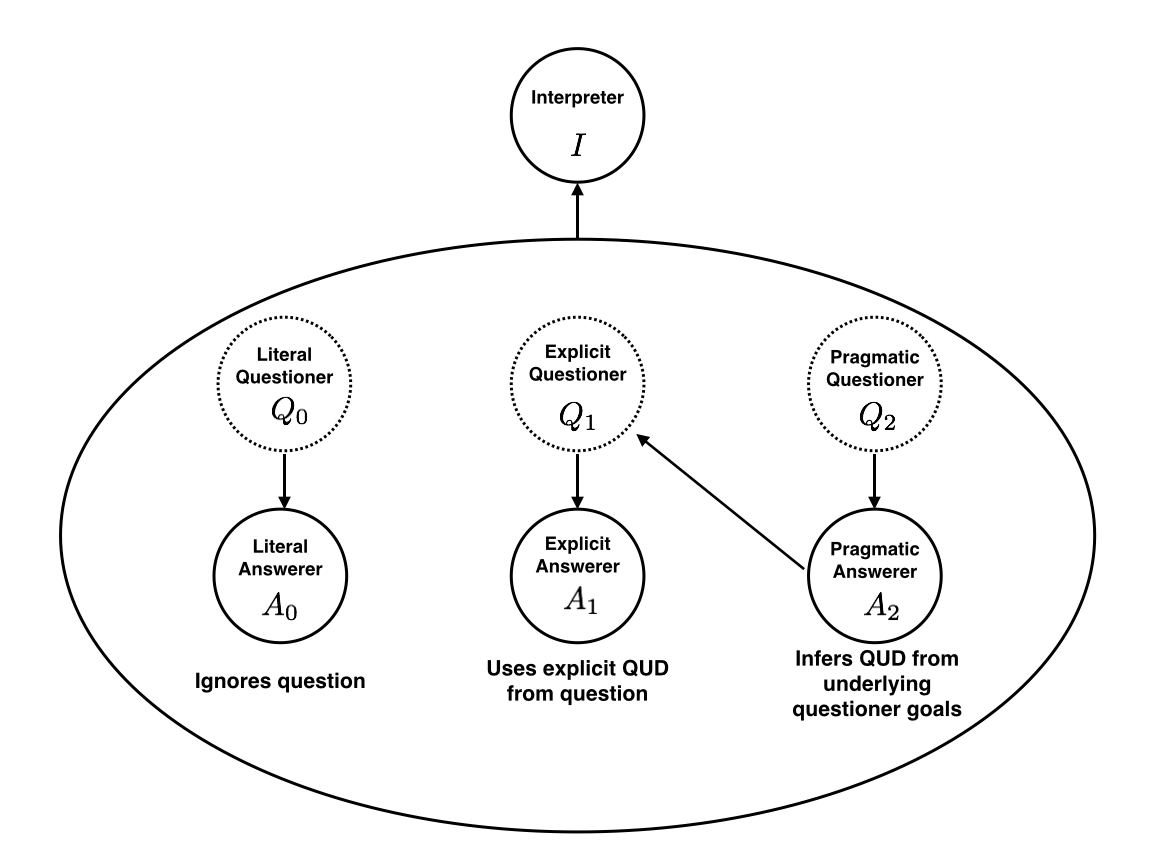
\includegraphics[scale = .75]{models.png}
\end{center}
\vspace{-.25cm}
\caption{Models.}
\label{fig:models}
\end{figure*}

More recent theories have tried to fix these problems by introducing some consideration of the questioner's goals. \citeA{VanRooy03_QuestioningDecisionProblems}, for instance, formalizes these goals as a decision problem faced by the questioner. A useful answer under this decision theoretic account is one that maximizes the expected value of the questioner's decision problem. A useful question is one that induces a sufficiently fine-grained partition, optimally distinguishing the worlds relevant to the decision problem. While this framework elegantly accounts for the context-dependence and relevance-maximization of question and answer behavior, it assumes that the questioner's decision problem is known a priori by the answerer. \todo{ndg: check.} If this were the case, the act of asking questions would seem irrelevant: why wouldn't the answerer directly tell the questioner which action to take?

Our models are an effort to expand on this core idea in a probabilistic framework, which also provides a mechanism for the answerer to \emph{infer} the `decision problem.' 
The RSA framework has already been applied to account for diverse pragmatic phenomena including scalar implicature\cite{GoodmanStuhlmuller13_KnowledgeImplicature}, 
interpretation of context-sensitive adjectives like ``tall'' or ``cheap'' \cite{LassiterGoodman15_AdjectivalVagueness}, 
non-literal language use like hyperbole \cite{KaoWuBergenGoodman14_NonliteralNumberWords} and irony \cite{KaoGoodman15_IronyCogSci}, 
and acquisition \cite{FrankGoodman14_InferringWordMeanings}. 
Our model situates question-answer behavior within this unifying view of language understanding as recursive social inference.

\section{A Rational Speech Act model of question and answer behavior}
\label{sec:model}

\subsection{Preliminaries}

Suppose there is a set of world states $\mathcal{W}$, 
a set of possible goals $\mathcal{G}$, 
a set of possible questions $\mathcal{Q}$, 
and a set of possible answers $\mathcal{A}$.%
%%%
\footnote{It is common in linguistics to distinguish between utterances and their underlying semantic values. In a complete language understanding model, we would have a separate space of question utterances $\mathcal{U}_q$ and a semantic evaluation function that maps a question utterance $u_q \in \mathcal{U}_q$ to its value in the semantic space $\mathcal{Q}$. Similarly, this evaluation function would map an answer utterance $u_a$ to its value in $\mathcal{A}$. For clarity, we assume these are trivial mappings and suppress them.}
%%%
These sets are taken to be in common ground between the questioner and the answerer. We formalize the notion of an informational goal $g \in \mathcal{G}$ as a projection function that maps a world state $w$ to a particular feature or set of features that the questioner cares about, which we denote $\hat{w} = g(w)$; this is similar to the notion of a question-under-discussion \cite<QUD;>{Roberts96_InformationStructureDiscourse}. QUDs are often used in formal linguistic models to capture \emph{relevance}: there are many informative sentences one can use to convey a full world state, but only a few of those are informative with respect to the current topic of discussion.

We will denote a distribution over the set of world states by $P(w)$, and will correspondingly use the notation $\widehat{P^g}(w)$ to indicate the probability of the $g$-projection of a world state $w$ under the projected distribution. Note that this is potentially very different from $P(g(w))$, the probability of the projected world state under the original distribution. Instead, 
$$\widehat{P^g}(v) = \int_{\mathcal{W}} \delta_{v=g(w)}P(w)dw$$ is a distribution over the image of $g$.

We must also specify the semantics we're using for questions and answers. We assume that the meaning of a question $q \in \mathcal{Q}$ is the same as that of a QUD: a projection from a world state to a feature (or features) of interest. This is equivalent to the more common partition semantics of \citeA{GroenendijkStokhof84_SemanticsOfQuestions}, as can be seen by considering the pre-image of such a projection: $q^{-1}(\hat{w})$. An answer is a map from world states to booleans, which eliminates possible worlds. This is equivalent to indicating a cell in the induced partition.

These semantics enter our model primarily through an \textbf{interpreter} function, which all agents use to compute the literal interpretation of an answer. The interpreter constrains the prior on worlds to the subset of its support that is consistent with the given answer:%
%%%
\footnote{For the purposes of this paper, we assume answers are always full sentences, corresponding to truth-functional propositions that can be evaluated in a given world. The interpreter describe is the simplest required to model such answers. For fragments such as `yes' or `Bob,' which can be used to answer questions like `Is dinner at 7pm?' or `Who got the promotion?' we would require a more sophisticated interpreter that can compositionally expand the fragment into a valid proposition, using the question. This is a standard operation in formal semantic models, and an interesting target for future research, but is not necessary for the experiments we report.}
%
$$P_I(w | a) \propto P(w) \delta_{a(w)}$$
%

\subsection{The Questioner}

How should a questioner choose between questions?
%
We start by assuming that the questioner aims to \emph{learn information relevant to a private goal}.
%
In order to choose a question that results in useful information, the questioner reasons about how the answerer would respond, given different possible states of the world; she selects a question that results in an answer that tends to provide goal-relevant information.
%

% This is a divergence from previous RSA models, where agents choose utterances with the goal of imparting information about the state of the world.

%\todo[inline]{i also think we should add subscripts of the different model components ($Q_0$, etc). should make a figure illustrating these components....

%we need to unpack and explain the math in this section more (since we have room in the long paper version).}

\newcommand{\KL}[2]{\ensuremath{D_{KL}({#1}\, \| \, {#2})}}
\newcommand{\E}[2]{\ensuremath{\mathbb{E}_{#1}\left [#2 \right]}}

More formally, the \textbf{questioner} takes a goal $g \in \mathcal{G}$ as input and returns a distribution over question utterances $q \in \mathcal{Q}$:
%
$$ 
P_{Q}(q|g)  \propto e^{ \E{P(w^*)}{\KL{\widehat{P^g}(w|q, w^*)}{\widehat{P^g}(w)}} - \,\,C(q)}
$$
%
It trades off the cost of asking a question, $C(q)$, and expected information gain. The expectation is taken over all possible true worlds $w^* \in \mathcal{W}$; we assume the questioner has uncertainty over which true world is actually the case (represented by the world prior $P(w^*)$). The cost likely depends on question length, among other factors. Information gain is measured as the Kullback-Leibler divergence between the ($g$-projected) prior distribution, $\widehat{P^g}(w)$, and the $g$-projection of the posterior distribution one would expect after asking a question $q$ whose answer reflected true world state $w^*$:
%
$$P(w|q, w^*) = \sum_{a \in \mathcal{A}} P_I(w | a) P_{A}(a| q, w^*)$$
%
%This conditional distribution reflects the fact that the answerer (who knows the true world state $w$) may behave noisily, have a limited set of possible answers, or other limitations.
%to questioner (who is inferring a world state $w^*$) is affected by stochastic answerer behavior and a limited set of possible answers. 
This distribution has two components: 
First, it depends on the interpreter, $P_I(w | a)$, which specifies the likelihood of different worlds after hearing an answer statement. Note this function does not depend on goals: we will only project along $g$ in the KL operator above after we have finished computed the posterior. Second, it depends on $P_{A}(a | q, w^*)$, a model of likely answerer behavior which we explore next.

\subsection{The Answerer}

How should an answerer choose between answers to a question? What should a questioner assume about the answerer when choosing a question? We next describe three different answerer models; the questioner could assume any one of them, leading to three corresponding versions of the questioner model. From here on, we index the questioner and answerer models by $i$ to formulate different questioner models $Q_i$ which reason about different answerers $A_i$ (see Figure \ref{fig:models}).
All answerers take a question $q \in \mathcal{Q}$ and a true world state $w^* \in \mathcal{W}$ as input and return a distribution over answers $a \in \mathcal{A}$.
%

The \textbf{literal answerer} simply chooses answers by trading off prior answer probability (interpreted here as cost) and how well that answer pair conveys the true state of the world to an interpreter:
%
$$P_{A_0}(a | q,w^*) \propto e^{P_I(w^* | \,a) - C(a)} $$
%
For a fixed question, this is equivalent to the speaker in previous RSA models. The question does not affect the response distribution, hence we do not expect it to be a very good explanation of question-answering phenomenon. It is of interest primarily as a null model for comparison to previous RSA models, where the speaker seeks to be informative without any queue from the listener.
%

The \textbf{explicit answerer} additionally evaluates answers with respect to how well they address the explicit question $q$. In other words, we use the question $q$ itself as the QUD projection, and choose answers proportionally to how well a listener with goal $q$ would guess the true state of the world $w^*$:
%
$$P_{A_1}(a | q, w^*) \propto e^{\widehat{P^q}_I(w^* | \, a) - C(a)}$$
This implements the simplest realistic theory of answerers: they attempt to reduce the questioner's uncertainty about the aspect of the world that they were queried about.

The \textbf{pragmatic answerer} also evaluates answers with respect to how well they address the questioner's goal, but doesn't take the question's explicit meaning at face value. Instead, the pragmatic answerer reasons about which underlying goals $g$ are likely given that a question $q$ was asked, and chooses answers that have high expected informativity:
%
$$
P_{A_2}(a | q, w^*) \propto e^{\sum_{g \in \mathcal{G}} P(g|q) \widehat{P^g}_I(w^*|\,a) - C(a)}
$$
Reasoning backwards from questions to goals is a simple Bayesian inversion of the (explicit) questioner using a prior on goals:
$$
P(g|q) \propto P_{Q_1}(q|g)P(g)
$$
We use the explicit ($i=1$) questioner model here for simplicity, but we could make $i$th order answerers that depend on the $(i-1)$th order questioner model, with arbitrarily high $i$. For the purposes of this paper, we will only examine the simplest $(i=2)$ pragmatic answerer, and the questioner that reasons about it -- as in previous studies using RSA models \cite<e.g.>{LassiterGoodman15_AdjectivalVagueness}, we do not find qualitative differences in the predictions of higher-order models.
%\todo[inline]{ndg: need to say here that we could depend on a sophisticated questioner model here, but we use the simplest(?) one for simplicity....}

For all of the questioner and answerer models, we can vary how strongly optimizing they are---that is, to what extent they are sampling from the distributions defined above, and to what extent they deterministically choose the most likely element. For any such distribution over utterances, we introduce an optimality parameter $\alpha$ and transform it by $ P'(x) \propto P(x)^{\alpha} $. Furthermore, we have set the answer prior in all answerer models such that outright false responses are excluded. The answerer models naturally assign very low, but non-zero probability to these options (because they are minimally informative). However, we set them to zero probability for the sake of simplicity in reporting and visualizing predictions.
%

This concludes our specification of the model space, giving a set of three answerers and three corresponding questioners that reason about them. We have implemented these models in WebPPL, a probabilistic programming language \cite{GoodmanStuhlmuller14_DIPPL}, and runnable code for all reported simulations is available online at \url{http://hawkrobe.github.io/Q\_and\_A/}. The model predictions shown throughout the rest of the paper are computed using this implementation. 

We emphasize that our models are situated firmly at the computational level \cite{Marr10_Vision} -- these models formalize hypotheses about the problem being solved by questioners and answerers in dialogue, and they make quantitative predictions about expected behavior under different assumptions. However, we do not propose that people are actively running a recursive probability calculation online every time they ask a question; further work is needed at the algorithmic and mechanistic levels to understand exactly what cognitive and neural processes give rise to the computations we predict. 

% Trying to frame the case studies section ("also, need to give more framing about what we're doing in this section and why. it's all about exploring the sensitivity of the answerer to plausible goals of the questioner, right?")
We now proceed to show how our model addresses four classic examples of question and answer pragmatics from the psycholinguistics literature. Because of the limited literature using questioner behavior as a dependent variable, all four examples explore the sensitivity of the answerer to plausible goals of the questioner. There are two primary benefits to re-formulating explanations from the original studies in our modeling framework: (1) the case studies are instructive as examples of how different components of the model interact to generate results and (2) by placing all four studies in a common framework, we more clearly see their commonalities.

\section{Four case studies}

\begin{table*}[t]
\centering
\begin{tabular}{ p{3cm} | r | r ||||||  r | r }
& \multicolumn{2}{c||||||}{Empirical} & \multicolumn{2}{c}{Model} \\
\hline
&           \% literal &   \%  info &           \% literal &   \%  info    \\
\hline
``Some bourbon'' &   0.37 & 0.63 &  0.38 & 0.62 \\
\hline
``Five dollars''     & 0.50 & 0.50 & 0.50 & 0.50 \\
\end{tabular}
\\[1.5pt]
\caption{Comparison of model predictions and data from Clark (1979). Shows the proportion of responses to the question ``Does a fifth of Jim Beam cost more than \$5?'' when paired with two contexts: ``I want to buy some bourbon'' (``Some bourbon'') and ``I've got \$5 to spend'' (``Five dollars''). } 
\label{table:clark79exp4}
\end{table*}

\subsection{Clark (1979), Experiment 4}
First, we show how our model can provide different---sometimes over- or under-informative---answers to the same explicit question, depending on context. For this illustration, we model the whiskey-pricing study presented in the Introduction \cite{Clark79_IndirectSpeechActs}. Recall that liquor merchants were more likely to give over-informative answers (specifying exact price) to the question ``Does a fifth of Jim Beam cost more than \$5?'' in the uninformative context (``I want to buy some bourbon'') than in the five dollar context (``I've got \$5 to spend'').

Our space of possible worlds consists of possible prices for the whiskey: $\mathcal{W} = \{\$1, \$2, \dots, \$10\}$. We consider two possible goals $g \in \mathcal{G}$: $g_=$, learning the actual price of whiskey,  and $g_>$, learning whether or not the agent can afford to buy the whiskey at all (i.e. whether the price is greater or less than \$5, the amount the agent has in their pocket). 

The set of answers $\mathcal{A}$ includes exact prices $a~\in~\{\$1, \$2, \dots, \$10\}$ as well as ``yes'' and ``no.'' The answer prior assigns equal probability to picking the category of ``yes/no'' answers and of ``price'' answers, then uniformly draws from the possible responses within each category. Thus, $$P(\textrm{``yes''}) = P(\textrm{``no''}) = 0.25$$ and $$P(\textrm{``\$1''}) = \cdots = P(\textrm{``\$10''}) = 0.05$$

Because the question was fixed in the experiment, the question space $\mathcal{Q}$ simply consists of the single question $q = $``Does a fifth of Jim Beam cost more than \$5?'' \todo[inline]{rdh: if we had alternative question possibilities, like ``How much does a fifth of whiskey cost?'', this would theoretically affect the pragmatic answerers' response: if they had been interested in the actual price, wouldn't they have asked the other question?} We model the context sentence as affecting the questioner's goal prior $P(g)$. When the context is ``I'd like to buy some whiskey,'' we assume that the the two goals are equally likely: $P(g_= | c) = P(g_> | c)$. When it is ``I only have \$5 to spend,'' we assume that it is more strongly in favor the agent learning whether or not they can afford it: $P(g_> | c)~=~.99$. We set the rationality parameter $\alpha = 1$.

%\todo[inline]{ndg: need to unpack these results -- this paragraph is quite cryptic.}

\subsubsection{Results} 

Our pragmatic answerer model's output is shown in Table \ref{table:clark79exp4}, compared with empirical results from \citeA{Clark79_IndirectSpeechActs}. The responses in \citeA{Clark79_IndirectSpeechActs} were tallied in three categories: literal answer only $(n_l)$, information only $(n_i)$, or both literal answer \emph{and} information $(n_b)$. For the purposes of this case study, we are only interested in the ratio of literal answers to information answers: $p_l = n_l/(n_l+n_i)$ and $p_i = n_i/(n_l+n_i)$.

Critically, our pragmatic answerer model displays the same context-dependence as the original empirical result: when the question is prefaced with ``I'd like to buy some whiskey,'', which makes the goal prior uniform across the two possible goals, then the correct exact price answer is favored more strongly (at probability $0.62$) than the literal response (probability $0.37$). This asymmetry arises in our model due to the fact that an exact price is much more highly informative than a literal response with respect to the ``exact price'' goal $g_=$, and if there is uncertainty over which goal is in fact the case, it is worth erring on the side of over-informativeness. This matches the empirical trend, which also favored the exact price answer (at probability $0.57$) over the literal answer (at probability $0.41$).

On the other hand, when the question is prefaced with ``I only have \$5 to spend,'' which makes the goal prior strongly favor the ``can I afford'' goal (with probability $.99$), then the model assigns equal likely to the literal and exact price responses. This arises because both responses are equally informative with respect to learning whether or not the agent can afford the whiskey, $g_>$, so the response likelihoods fall back to the answer prior. This also matches the empirical trend, where the exact price and literal answer were equally likely.

Note that the literal and explicit answerers (which have no natural way to account for context) do not make different predictions in the two contexts. The literal model predicts that the answerer is equally likely to say the true Boolean answer and the true numerical answer, and the explicit model predicts that the answerer will always give the true Boolean answer, since it is the explicit question being asked. This suggests that our pragmatic \emph{answerer} is consistent with human behavior in psychologically interesting situations, passing a first, qualitative, test. 

\subsection{Groenendijk and Stokhof (1984)}
 \begin{figure*}[t!]
\begin{center}
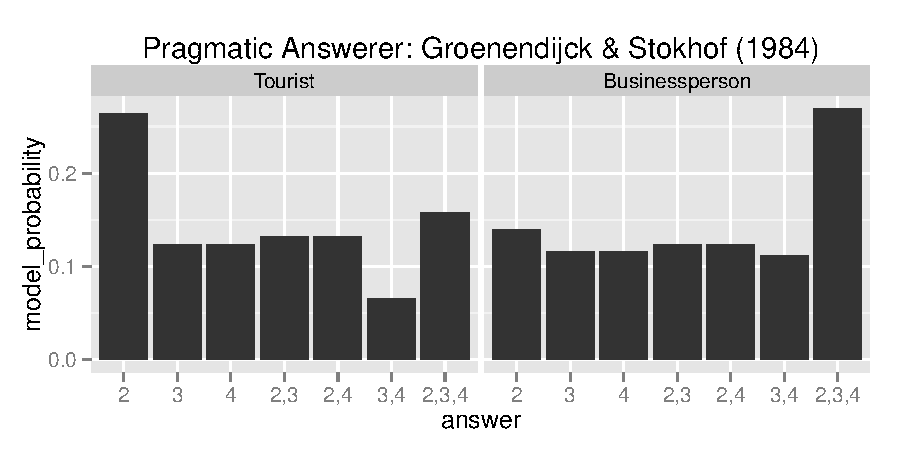
\includegraphics[scale = 1]{groenendijckPlot.pdf}
\end{center}
\vspace{-.25cm}
\caption{Results for our computational experiments implementing the Groenendijck \& Stokhof (1984) \emph{mention-some} problem.}
\label{fig:cafeExperimentResults}
\end{figure*}

For a slightly more complex example, we consider the classic puzzle of \emph{mention-some} and \emph{mention-all} readings of wh-questions  \cite{GroenendijkStokhof84_SemanticsOfQuestions}. Some \emph{wh-}questions, like ``Who is coming to dinner tonight?'' are intended to elicit an exhaustive list of the entities that are answers. For ostensibly similar questions, like ``Where can I find a bathroom in this building?'', a single answer would be sufficient. Many recent theoretical explanations in the linguistics literature appeal to questioner goals \cite<e.g.>{SchulzVanRooij06_ExhaustiveInterpretation, Ginzburg95_ResolvingQuestions}. While there are no experimental results on \emph{mention-some} and \emph{mention-all} readings with which we can compare our model's output, we include the phenomenon as a case study for its value in demonstrating how our model formalizes the standard explanation. 

We focus on a question like ``Where do they sell Italian newspapers in Amsterdam?'' that can intuitively be ambiguous between these meanings depending on who is asking: if it is a tourist, they probably just want to know the nearest place, but if it is a businessperson trying to build a newspaper distribution network, they likely want the whole list \cite<see>{GroenendijkStokhof84_SemanticsOfQuestions}. The puzzle is determining how the same question can take on different meaning in different contexts: according to our account, this happens via an inference about the questioner's underlying goal.

Our world space $\mathcal{W}$ consists of all possible assignments of properties to a set of four cafes in town. Each cafe has two properties: its distance from the speaker and whether or not it sells Italian newspapers. There are two possible goals (or QUDs) $g \in \mathcal{G}$: $g_{n}$, learning the identity of the \emph{nearest} cafe selling a newspaper, and $g_{a}$, learning the identity of \emph{all} cafes selling a newspaper. Both of these are represented by projections on world states, mapping a list of cafes to the single cafe selling newspapers with the lowest distance or to the sublist that sell newspapers, respectively. The space of answers $\mathcal{A}$ includes all $\sum_{i=0}^4 {4 \choose i} = 16$ combinations of different cafes (e.g. ``none,'' ``cafe1,'' ``cafe 1 and cafe 3,'' or ``cafe 2, cafe 3, and cafe 4''). Again, our question space $\mathcal{Q}$ consists of a single question: ``Where can one buy an Italian newspaper?''

For the prior $P(a)$ over answer utterances, we use a (truncated) geometric distribution, which is common over spaces where probabilities should naturally scale with some count. Let $\ell(a)$ be the number of locations named in the answer (e.g. $\ell(\textrm{`none'})~=~0, \ell(\textrm{`cafe 1'})~=~1$, etc). Then the probability of an answer $a$ is given by:

$$P(a) \propto \frac{(1 - p)^{\ell(a)}p}{{4 \choose (\ell(a))}}$$
which we re-normalize to account for the fact that $\ell(a) \le 4$ for all $a\in \mathcal{A}$. In our computational experiment, we fix $p = 0.6$. 
This simple distribution has two advantageous properties: 
\begin{enumerate}[(1)]
\item the probability mass assigned to a given length by the geometric distribution is spread evenly across different answers of that length.
\item we naturally assign longer answers lower probability, reflecting their higher cost of utterance. \end{enumerate}

We model the context sentence as affecting the questioner's goal prior $P(g)$: if they say ``I'm new here,'' then there's a high chance that they are interested in the closest location with a newspaper ($P(g_n | c) = 0.9$); if they say ``I'm a businessperson\dots,'' then there's a high chance that they are interested in all of the newspaper locations ($P(g_a | c) = 0.9$).\footnote{Note that this formulation of the problem differs slightly from the one given by \citeA{GroenendijkStokhof84_SemanticsOfQuestions}, although they easily map onto one another. In the original formulation, the \emph{answer} is fixed and the \emph{meaning} of the answer must be inferred to either be mention-some or mention-all. In our formulation, the meaning of each answer is unique and fixed, but the answerer must choose among a set of different possible answers. The same inferential machinery that our questioner uses to reason about which answer utterance the answerer will give could also be used to reason about which \emph{meaning} the answerer intends by their fixed utterance. The only difference is that the questioner would have uncertainty over a set of possible meanings instead of uncertainty over a set of possible answer utterances. We chose the latter because it more closely resembles the other scenarios we are modeling.}

It remains unclear where these goals and goal priors may come from in real-world situations: it is likely tied to background knowledge about tourists, newspapers, and the business world, as well as past experience in social situations. While these deeper explanations lie outside the scope of our model, we still have explanatory power in showing how goals interact with other terms, and how the prior differ across scenarios. 

 \begin{figure*}[t!]
\begin{center}
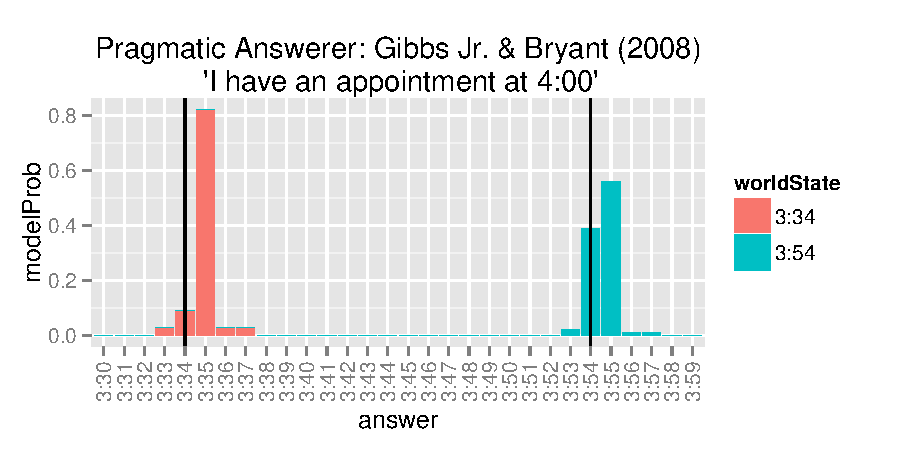
\includegraphics[scale = 1]{timeExpResults.pdf}
\end{center}
\vspace{-.25cm}
\caption{Results for our computational experiments replicating Gibbs Jr. and Bryant (2008). Vertical lines represent the true world state.}
\label{fig:timeExperimentResults}
\end{figure*}

\subsubsection{Results}

For concreteness, we set the true world to be the following :

\begin{lstlisting}
world = {`cafe1' : [3, false],
         `cafe2' : [1, true],
         `cafe3' : [3, true],
         `cafe4' : [3, true]}
\end{lstlisting}
meaning that `cafe1' is three blocks away from the speaker and does \emph{not} sell Italian newspapers, `cafe2' is one block away and \emph{does} sell Italian newspapers, and so on. We enumerated over all model executions for both contexts. Results are displayed in Figure \ref{fig:cafeExperimentResults}. We find that the highest probability response given the ``tourist'' context is the single location ``cafe2,'' with response probability $p = 0.26$. This is in fact the nearest location selling newspapers, informatively fulfilling the contextually more likely goal $g_n$. Note that responses containing ``cafe1'' are ruled out entirely, as it does not carry Italian newspapers. Of the remaining responses, those including ``cafe2'' have relatively higher probability, while ``cafe3, cafe4'' is assigned lowest probability, as it does not informatively address \emph{either} goal and is also relatively unlikely under the prior. 

Given the ``businessperson'' context, however, the highest probability response is the conjunction ``cafe2 and cafe3 and cafe4,'' with probability $p = 0.27$. This is the exhaustive answer, informatively fulfilling the contextually more likely goal $g_a$ of knowing the location of all cafes selling Italian newspapers. The remaining answers are equally unlikely, as they all fail to be informative about the exhaustive list of locations. The slight variability, with $a = `cafe2'$ more likely than the rest, and $a = `cafe3, cafe4'$ less likely, is due to the influence of the less likely ``nearest'' goal, and the answer prior.

The literal and explicit answerers, as in the Clark scenario, do not have the means of making inferences about the questioner's underlying goals. Thus, both models incorrectly predicted that the context would not affect the preferred response. The literal answerer predicted that all combinations of cafes 2, 3, and 4 would be given in proportion to their prior likelihood (with no special preference given to the closest one). The explicit answerer predicted that the exhaustive answer would be preferred in all contexts (as this is literal semantics we encoded for the question).  Crucially, the only difference between our model of this scenario and the Clark scenario is the space of QUDs, the structure of the world, and the meanings of the answers. The questioner and answerer functions stayed exactly the same.
%%%%


\subsection{Gibbs Jr. \& Bryant (2008): Experiment 3}

It has been shown in previous work that people typically round their answers to the nearest 5 minute interval when asked `Do you have the time?'', even when they're wearing a digital watch \cite{DerHenstCarlesSperber02_RelevanceTellingTime}.  \citeA{GibbsBryant08_OptimalRelevance} replicated this result, and then performed a follow-up study on analog-watch wearers where they preceded their question by the context ``I have a meeting at 4:00.'' 

They found that the tendency to round times decreased as a function of the time remaining until the stated deadline: the group asked 30-16 minutes before the stated appointment rounded their responses 79\% of the time, while the group asked 14 minutes or closer to the appointment rounded significantly less (62\%). They explained this result by appealing to the questioner's goals: while an approximate time is sufficiently informative with respect to most goals, such as knowing how much time is left before heading to an appointment, a questioner who is running late may need to gauge how quickly they should move, whether they should call and warn about being late, or make other such decisions, in which case a precise time is highly relevant. 
\begin{table*}[t]
\centering
\begin{tabular}{ p{2cm} | r |||||| r }
&  \% round (Empirical) &  \% round (Model) \\
\hline
Early group &  0.79 & 0.77 \\
\hline
Late group     &0.62  & 0.60 \\
\end{tabular}
\\[1.5pt]
\caption{Comparison of our model predictions with data from Gibbs Jr. and Bryan (2008). Shows the proportion of rounding in response to ``I have an appointment at 4:00. Do you have the time?'' for two groups: an ``early group'' where the appointment was in 30-15 minutes and a ``late group'' where the appointment was in less than 15 minutes.} 
\label{table:gibbsJrExp3}
\end{table*}
To set up this scenario in our model, we take the world space to be the set of possible times, which we limit to a half hour interval (as in the experiment): $\mathcal{W}~=~\{\textrm{3:30}, \textrm{3:31}, \dots, \textrm{3:59}\}$. Unlike in the previous two case studies, where there were only two contrasting goals and two contexts that make each goal more or less likely, we now use a larger, parametrized goal space and a single context stating the time of the appointment that is held fixed across different conditions of the experiment. 

This goal space $\mathcal{G}$ includes the trivial projection $g_0(w) = w$, corresponding to the context-independent goal of learning the true time, in addition to a set of goals parameterized by a threshold time $\tau$, representing the point at which the agent believes they are running late to their appointment (likely based on expectations about travel time, social norms concerning lateness, and other exogenous factors). If the agent has goal $g_\tau$ for a given $\tau$, then for times $t < \tau,$ the agent only cares about the approximate time, rounded to the nearest 5 minute increment, in order to know roughly how much time they have before leaving. For times $t > \tau$, the agent cares about the exact time in order to make the kind of decisions described above. Formally,

\DeclarePairedDelimiter{\floor}{\lfloor}{\rfloor}

$$g_\tau(w) = \left\{
\begin{array}{rcl}
w & & w \ge \tau\\
5\floor{\frac{w}{5} + \frac{1}{2}} & & w < \tau;  \\
\end{array}
\right.
$$
where $\floor{w}$ returns the \emph{floor} of an integer and all operations are assumed to act on the minutes component of a time $w$. For example, the goal $g_{3:50}$ with the threshold set at $\tau = $3:50 corresponds to a projection function that rounds input worlds earlier than 3:50 and does not round worlds later than 3:50. This would be the case if the agent knew they would need to leave around 3:50 in order to make it to an appointment on time. 

The goal prior $P(g_\tau)$ assigns probability $p=0.25$ to the context-independent goal $g_0$ of wanting to know the exact time. The remaining probability mass is divided across different threshold goals ($\tau \in \{$ 3:31, 3:32, \dots, 3:59 $\}$) according to the following rule: the likelihood of each goal $g_\tau$ is inversely proportional to the distance (in minutes) between the threshold $\tau$ and the given appointment time $c$, reflecting the intuition that the questioner will be more likely to be running late, and therefore in need of the exact time, as it approaches the appointment time:

$$P(g_0) = 0.25$$
$$P(g_\tau; c) = \frac{0.75}{\sum_{i=1}^{29}i}(30 - |\tau - c|)$$

\todo[inline]{rdh: This would be cleaner if we could leave out the normalization constant... But just using $\propto$ isn't technically correct, since it's important to normalize accounting for the flip$(0.25)$ division between the pure goal and the threshold goals}
The set of answers is the set of times that could be given (e.g. 3:30, 3:31, \dots, 4:00), with multiples of 5 preferred:
$$P(t) = \left\{
\begin{array}{lcl}
0.125 & & t \equiv 0 \mod 5 \\
0.01 & & \textrm{otherwise} \\
\end{array}
\right.
$$ As \citeA{GibbsBryant08_OptimalRelevance} point out, their participants all wore analog watches, hence precise answers have higher cost. In fact, an earlier study in the same paper showed that in the absence of any context, participants wearing analog watches responded with rounded answers 90\% of the time, so this prior is realistic. 

For our answers, we use exact number semantics: the response ``3:35'' evaluates to true in worlds where the time is in fact 3:35, and false otherwise. While we suppressed \emph{a priori} false answers for convenience in other case studies (they would be naturally be assigned vanishingly small probability anyway), note that we cannot do so here: answerers must be allowed to make \emph{a priori} false utterances that get reinterpreted by the listener to be true under the QUD \cite<see>{KaoWuBergenGoodman14_NonliteralNumberWords}.

 \subsubsection{Results}
 
To compare our model's performance against the `early group' and `late group' conditions in \citeA{GibbsBryant08_OptimalRelevance}, we ran two simulations. In both, the context is ``I have an appointment at 4:00.'' In the first, the true world state is between 3:30 and 3:45 (the `early' condition); in the second, the true world state is between 3:45 and 3:59 (the `late' condition). In each condition, we ran our pragmatic answerer model for all true worlds in the appropriate range of times, and report the average probability of responding with a rounded answer. Our results are compared against empirical data from Gibbs Jr. and Bryant \citeyear{GibbsBryant08_OptimalRelevance} in Table \ref{table:gibbsJrExp3}. 

To more closely analyze what is driving our model's performance in these two conditions, we examine the answer behavior for two specific world states: one from the `early group' (3:34) and one from the `late group' (3:54). Answer probabilities for these two conditions are shown in Figure \ref{fig:timeExperimentResults}. We found that our pragmatic answerer model rounds the 3:34 to 3:35 in the `early' condition with probability $p = 0.74$, but rounds 3:54 to 3:55 with lower probability $p = 0.65$ in the `late' condition. 

The goal prior is the key component of the model governing this difference. Note that that (1) \emph{all} states in the pre-image of the rounding projection from the true time $t_0$ are assigned lower probability than the rounded time $g_\tau(t_0)$, due to the influence of goals $g_\tau$ with thresholds $\tau > t_0$ and (2) the true time $t_0$ is assigned relatively higher probability than the other non-rounded times, due to the influence of the pure goal $g_0$ and goals $g_\tau$ with thresholds $\tau < t_0$. This dynamic, paired with the upward-skewed prior on goal priors discussed above, causes the `late' condition to assign a much higher relative probability to the true time, than the `early' condition.

The pragmatic answerer thus accurately captures the empirical results both qualitatively and quantitatively. Our literal and explicit answerer models fail to capture these contextual differences, as they do not reason about the space of underlying goals (which justify rounding) and always give the exact time. The literal answerer always gives the exact time because it is the only property of the world, which they are attempting to be informative about without regard to the question. The explicit answerer always gives the exact time because it uses the explicit question meaning, which simply asks for the time.

\todo[inline]{rdh: Actually, in the experiment the question was ``Do you have the time?'' to which the literal and explicit answers would be ``yes'' or ``no'', right? We don't allow these responses in our model because they're not what we're interested in (i.e. \emph{no one} responded this way), but they are the kinds of answers our literal and explicit answerers would give}


\todo[inline]{rdh: Discuss the fact that we clearly set some numbers to get a good quantitative fit, specifically the base likelihood of the pure goal in the goal prior (0.25) and the likelihood of rounded answers vs. non-rounded answers in the answer prior (0.75)?}
\begin{table*}[t!]
\centering
\begin{tabular}{ p{5cm} | r | r ||||||  r | r }
& \multicolumn{2}{c||||||}{Empirical} & \multicolumn{2}{c}{Model} \\
\hline
&           \% literal &   \%  info &           \% literal &   \%  info    \\
\hline
``Master Charge cards?'' &   1.00 & 0.00 &  0.92 & 0.08 \\
\hline
``American Express cards?''     & 1.00 & 0.00 & 0.96 & 0.04 \\
\hline
``Credit cards?''     & 0.73 & 0.27 & 0.76 & 0.24 \\
\end{tabular}
\\[1.5pt]
\caption{Comparison of model predictions and data from Clark (1979), Experiment 5. Shows the proportion of literal and over-informative responses restauranteurs gave to each of three different questions from a customer inquiring about credit cards.} 
\label{table:clark79exp5}
\end{table*}

\subsection{Clark (1979): Experiment 5}
Our final scenario demonstrates the role of the questioner component in our pragmatic answerer model. Because the question space in the previous computational experiments only contained one element (by virtue of the task being modeled), the pragmatic answerers' inferences were entirely based on the context and the QUD prior. One of the most interesting and novel predictions of the RSA model, however, is that the questioner's choice of utterance itself should guide a pragmatic answerer's inferences about likely underlying goals. While there are few previous experimental results using questioner behavior as the \emph{dependent variable}, there is some work manipulating the question asked as an \emph{independent variable} and testing how it affects answers.

One such study was conducted as a follow-up to the first experiment we modeled earlier in this paper.  \citeA{Clark79_IndirectSpeechActs} called restaurants and asked one of four yes/no questions about which \emph{credit cards} the restaurant accepted:

\begin{enumerate}
\item ``Do you accept Master Charge cards?'' 
\item ``Do you accept American Express cards?''
\item ``Do you accept credit cards?'' 
\item ``Do you accept any kinds of credit cards?'' 
\end{enumerate}

He analyzed the likelihood that the respondent gave a literal yes/no answer, compared to the likelihood of giving the full (over-informative) list of exactly which cards were accepted.  He found that (1) and (2) were nearly always answered with a `yes' or `no', (3) was slightly more likely to be answered with full information, and (4) was \emph{much} more likely to be answered with full information (see Table \ref{table:clark79exp5}). As in the first case study above, we are only interested in the ratio of literal answers vs. over-informative answers $p_l = n_l/(n_l + n_i)$ and $p_i = n_i/(n_l + n_i)$, not in responses including both. We restrict our analysis to the first three questions\footnote{We view Clark's results for the fourth question as an example of M-implicature: by using a more costly utterance with the same literal meaning as question (3), the meaning of (4) becomes marked. Rational speech act models capture M-implicature by introducing \emph{lexical uncertainty} \cite{BergenGoodmanLevy12_Alternatives}, where both speaker and listener begin their inference with uncertainty over the literal meaning of utterances. By jointly reasoning about an utterance's meaning and the world state the speaker is trying to convey, more costly utterances are mapped to meanings with lower prior probability, allowing a pragmatic inference that ``Do you accept any kinds of credit cards?'' most likely means something like ``What kinds of credit card do you accept?'' Because this is the only example of M-implicature that arises in this paper, and it is not even the critical result from the experiment we are modeling, we believe that a presentation of the full lexical uncertainty model would be unnecessary and confusing to the reader.}.

We formalize Clark's analysis of the scenario in our model in the following way. The set of possible worlds $\mathcal{W}$ is given by the power set $\mathcal{P}(\mathcal{C})$, where $\mathcal{C} = \{$Visa, Master Card, American Express, Diner's Club, and Carte Blanche$\}$, the set of five possible credit cards. This power set contains all $2^5 = 32$ subsets of cards that the restaurant might accept. The prior distribution over worlds, $P(w)$, takes into account the true likelihoods of restaurants accepting different cards. Clark reports these likelihoods to be 72, 71, 38, 12, and 10\% for Visa, Master Card, American Express, Diner's Club, and Carte Blanche, respectively. 

The question space $\mathcal{Q}$ contains the five basic questions (``Do you accept $c$?" with $c \in \mathcal{C}$ one of the five cards) in addition to ``Do you accept credit cards?'' For the literal semantics of the five basic questions, indexed by $c$, we use the projection 
$$g_c(w) = \left\{\begin{array}{rcl} 1 && c \in w \\ 0 && \textrm{otherwise}\end{array}\right.$$ 
therefore partitioning the space of possible worlds into one cell  in which card $c$ is accepted and another cell in which it is not. The latter question returns \texttt{true} on worlds that accept at least one card and \texttt{false} otherwise: 
$$g(w) =  \left\{\begin{array}{rcl} 1 && |w| > 0 \\ 0 && \textrm{otherwise}\end{array}\right.$$ 
The prior distribution $P(q)$ over these questions is proportional to question length, which happens to be uniform.

The answer space $\mathcal{A}$ contains `yes', `no', and all possible combinations of the five cards. Thus, the restauranteur could respond to the question ``Do you accept Master Charge cards?" by saying ``Yes'' or by saying something like ``We accept Visa and Diner's Club." As in our early case study of Clark's (1979) whiskey experiment, we assign prior probability $p = 0.5$ to ``yes''/``no'' type responses, and prior probability $p = 0.5$ to card type responses, with uniform distributions within each category. To simplify our analysis, we have our agent restrict their prior to responses which are both \emph{true} (e.g. they would not say ``We accept Visa'' when they only accept American Express) and \emph{exhaustive} (e.g. they wouldn't  say ``We accept Visa'' when they accept Visa and three other cards). This corresponds to the way Clark (1979) classified responses. 

Finally, all goal projections $g \in \mathcal{G}$ correspond to solving a simple problem: finding out whether the restaurant accepts one of the cards they own. This family of goals is parametrized by $\mathcal{C}_q$, the set of cards that the questioner actually owns, with a prior $P(g)$ using the same likelihoods that govern the world prior\footnote{This corresponds to an assumption that restaurants accept cards proportional to the percentage of people owning those cards. This assumption was suggested by Clark (1979), but not used in his informal analysis).}. Formally, for the goal $g_{\mathcal{C}_q}$, we define a projection on worlds $w$, which maps a world to \texttt{true} if they accept at least one of the cards in $\mathcal{C}_q$ and \texttt{false} otherwise. 

$$g_{\mathcal{C}_q}(w) = \left\{\begin{array}{rcl} 1 && | \mathcal{C}_q \cap w | > 0 \\ 0 && \textrm{otherwise}\end{array}\right.$$
 \begin{figure*}[t!]
\begin{center}
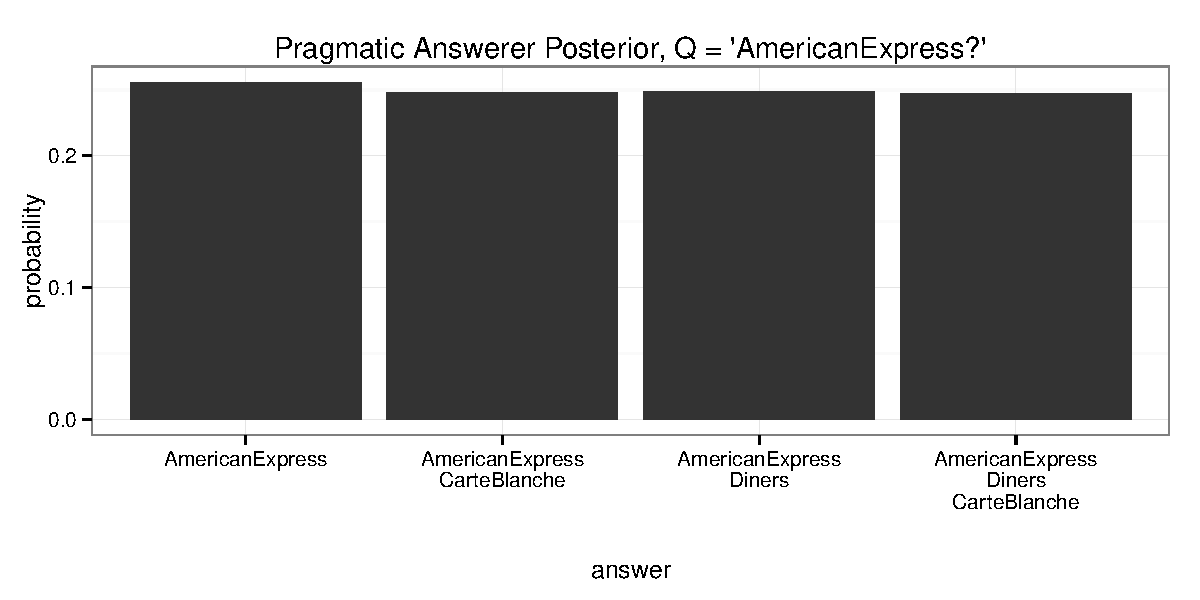
\includegraphics[scale = .6]{americanExpressPosterior.pdf}
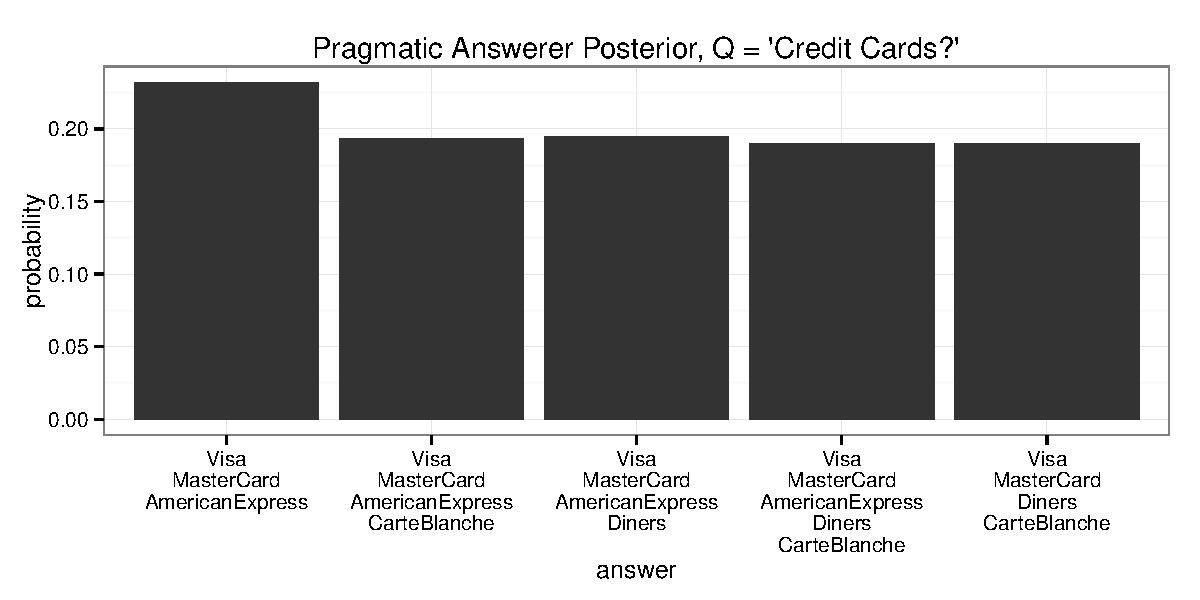
\includegraphics[scale = .6]{creditCardsPosterior.pdf}
\end{center}
\vspace{-.25cm}
\caption{Comparison of questioner goal posteriors that the pragmatic answerer model infers after hearing two different question utterances in Clark (1979), Experiment 5.}
\label{fig:clarkExperiment5posteriors}
\end{figure*}

\subsubsection{Results}

For each possible question in the experiment, we tested the likelihood of our pragmatic answerer responding with a literal ``yes''/``no'' vs. an exhaustive list of accepted cards, marginalizing over all possible world states. For quantitative fit, we tuned a single rationality parameter $\alpha$, shared by all model components. For the results presented in Table \ref{table:clark79exp5}, we found the best quantitative fit when $\alpha \rightarrow \infty$. We use $\alpha = 10000$, since the predictions stabilize above this value. Recall that a high value of $\alpha$ corresponds to an agent that maximizes with respect to their probability distribution (i.e. always picks the utterance with highest probability, which is technically optimal)\footnote{Note that while we use deterministic QUDs for all scenarios in this paper, our implementation of the model in a probabilistic programming language makes it just as easy to use \emph{probabilistic} projections: mappings that partition the world space in different ways with different probabilities. If we instead use a family of goals $\mathcal{G}$ that samples uniformly from the set of cards owned and project to 1 on worlds that contain \emph{that card}, then we achieve the same results with a much lower $\alpha$. Probabilistic QUDs are currently non-standard in the semantics literature, and it will be interesting in future work to test the extent to which they provide a better pragmatic model}. 

We find that when the questioner asks ``Do you accept MasterCard?'', the pragmatic answerer gives a literal ``yes''/``no'' answer with probability $p = 0.92$ (compared to $p=1.00$ empirically). Similarly, when the questioner asks ``Do you accept American Express?'', the pragmatic answerer gives a literal answer with probability $p = 0.96$ (also compared to $p=1.00$ empirically). The small difference between these predicted response probabilities comes from the relative likelihoods of the different cards in the true world. However, when the questioner asks ``Do you accept credit cards?'', the probability of a literal response drops to $p = 0.76$ (compared to $p=0.73$ empirically). Our model output therefore provides a good fit to the original experiment data, both qualitatively and quantitatively.

To further understand \emph{why} our pragmatic answerer model behaves this way, we can examine the posterior over questioner goals that the pragmatic answerer infers from each question utterance (see Figure \ref{fig:clarkExperiment5posteriors}). First, suppose they hear the question ``Do you accept American Express?'' We see that the pragmatic answerer rules out all but four goals, all of which consist of the questioner owning an American Express card and possibly a less common card. 

This is because (1) an explicit questioner who owns any more common cards would ask about the most common one instead ($\alpha$ is high, so a question about a more common card is slightly more likely to get a positive and therefore resolving answer from the explicit answerer -- when maximizing, the agent picks the slightly better option 100\% of the time) and (2) an explicit questioner who doesn't own an American Express card would not learn much from hearing whether or not this card is accepted. 

Having inferred this goal distribution, the pragmatic answerer then reasons that a literal response of ``yes'' (if true) perfectly rules out possible worlds in which the merchant does \emph{not} accept American Express, informatively resolving the question. Giving an exhaustive list of accepted credit cards is still a valid answer, but useful only in a small number of worlds (e.g. where American Express is not accepted but Carte Blanche and/or Diner's card \emph{are} accepted).

When asked "Do you accept credit cards?'' the pragmatic answerer reasons via Bayesian inference that the questioner's goal is \emph{not} solely to find out whether a single card $c \in \mathcal{C}$ is accepted. If this was their goal, they would have asked the more direct question ``Do you accept card $c$?'' and because they did not ask this question, it must not have been the goal. This inference also rules out goals where the questioner has one common card $c$ plus one or more rarer cards, since these goals also lead to the question ``Do you accept card $c$?'' 

With all these goals ruled out, we are left with five goals in which the caller has \emph{both} common cards (Visa and MasterCard) along with various other less common cards. The answerer is uncertain as to which set of less common cards are owned. Thus, for any world where the restaurant does not accept Visa or MasterCard, an exhaustive list of accepted cards is determined to be the most informative answer on average. Note that these inferences are made purely on the basis of the questioner model's behavior under possible goals, rather than cues from context as in the previous simulations.

\subsection{Discussion}

Our question-asking and answering model reproduced quantitative and qualitative patterns of question-answer behavior in four different scenarios from the psycholinguistics literature. It captured both explicit and implicit context effects as well as effects where the question itself served as a signal about the relevant underlying goals. In all cases, we found that our pragmatic answerer was required: without taking into account context or the questioner's underlying QUD, the explicit answerer is unable to adapt their response to different circumstances as experiments found.

\todo[inline]{rdh: thought I should lampshade in the next $\P$ the fact that our models have 0.5s here and 0.75s there, with no good explanation for where those numbers come from, and offer an argument for why this shouldn't be too worrying -- not sure if we need this, or whether this is the right place to put it, though}
One salient issue with our computational experiments is that our resulting answer distribution depends in each case on hard-coded settings such as the space of alternative questions, answers, and goals and the mathematical form of the various priors. We set these components to be simple and natural in the context of the scenario being modeled, but there is still some concern over the amount of flexibility afforded to the modeler in making these choices. For example, the answer prior for both Clark studies uses a parameter to determine the answerer's baseline preference for `yes' and `no' responses versus prices or lists of card types. In both cases we set this parameter to be $p = 0.5$, but other numbers could have been chosen to achieve a better or worse quantitative fit. 
\begin{figure}[t!]
\begin{center}
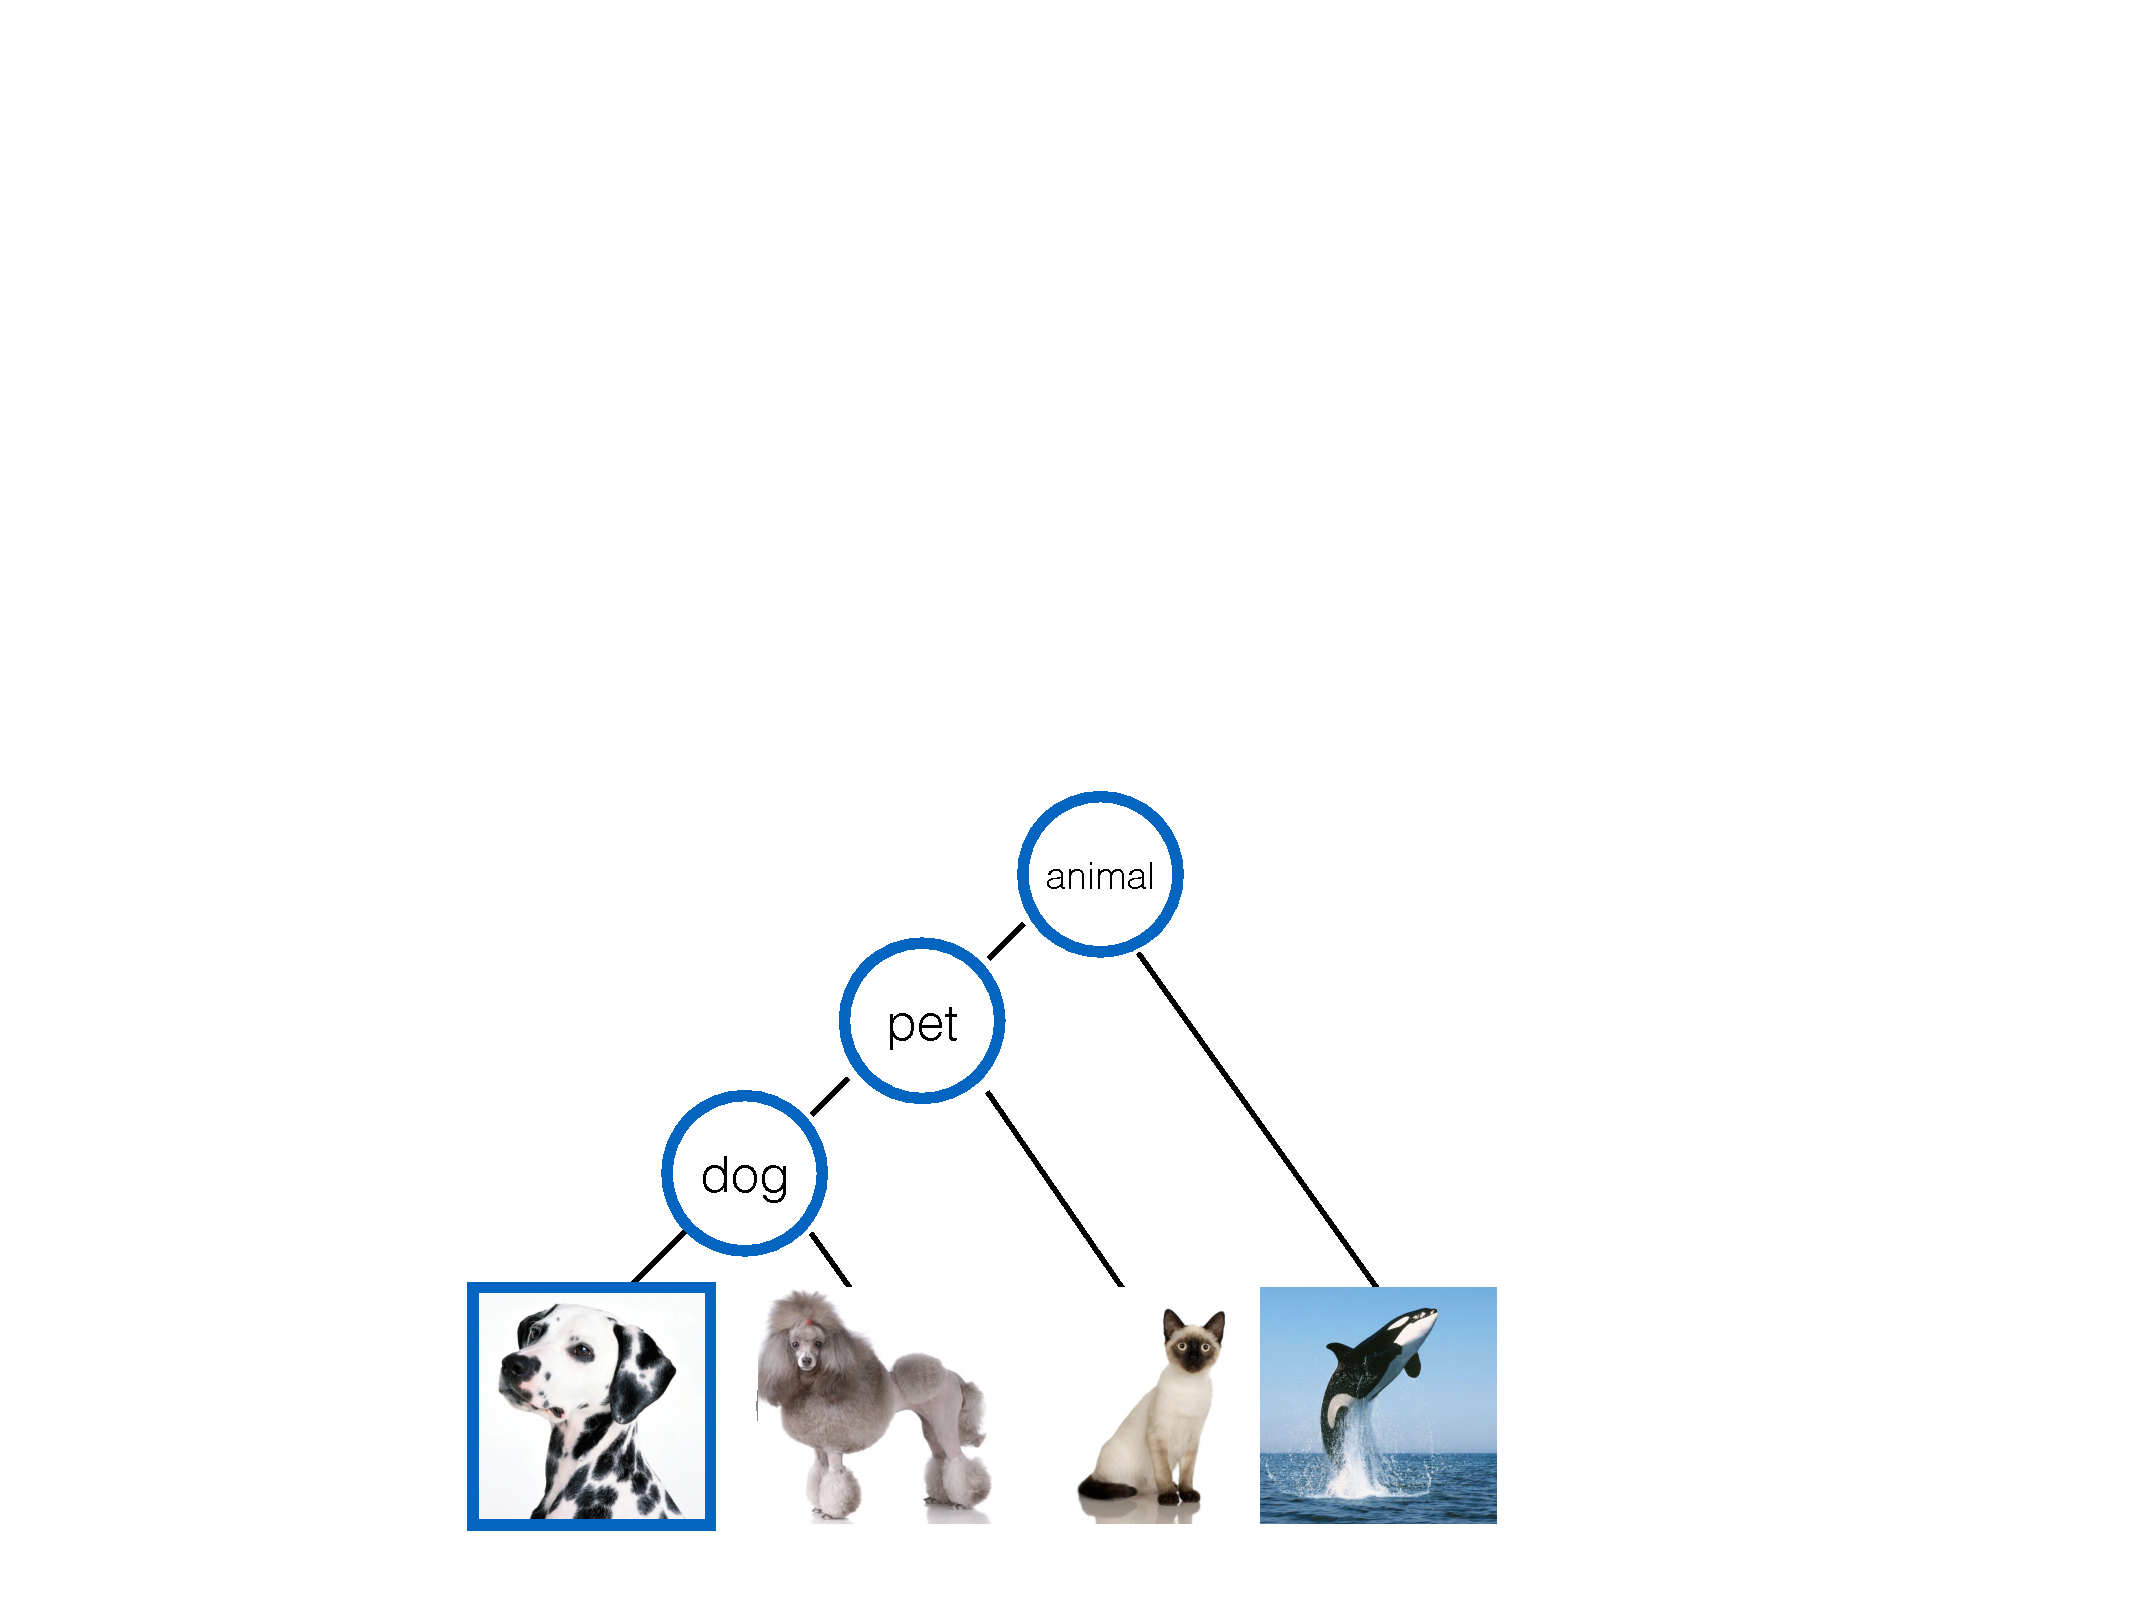
\includegraphics[scale = .35]{taskhierarchy.pdf}
\end{center}
\vspace{-.25cm}
\caption{Stimulus hierarchy used in Exp.~1. The goal space and answer space contained the four leaves. %hidden behind gates (the nodes of the tree). 
The question space, however, was restricted to the highlighted nodes, proceeding up the hierarchy, allowing for indirect questions.}
\label{fig:taskhierarchy}
\end{figure}

This raises concerns that our model could fit \emph{any} question-answer data by choosing the appropriate set of priors. Indeed, we regard all of these choices as scientific hypotheses, not free parameters. For the experiments presented later in this paper, we test these hypotheses or fix them via our experiment design. The choices in the computational experiments above were simply intended to be reasonable enough to illustrate how our model framework accommodates various results from the literature on question-answer pragmatics.

\todo[inline]{rdh: Could put in a $\P$  here about why we're testing literal and explicit models at all since they suck so much}
While the questioner component of our model was critical to the pragmatic answerer's behavior in the final simulation, none of these scenarios truly tested the questioner component.  Indeed, most empirical work has treated the question or context as an independent variable, with the answer as a dependent variable. Our model, following \citeA{VanRooy03_QuestioningDecisionProblems}, however, suggests that the question itself is important in prompting a relevant answer, hence questioner behavior should be treated as a dependent variable. In order to test these predictions, we designed a sequence of experiments using a communication game to collect data on both question-asking behavior \emph{and} question-answering behavior.

%%%
%
	\begin{figure*}[t!]
\begin{center}
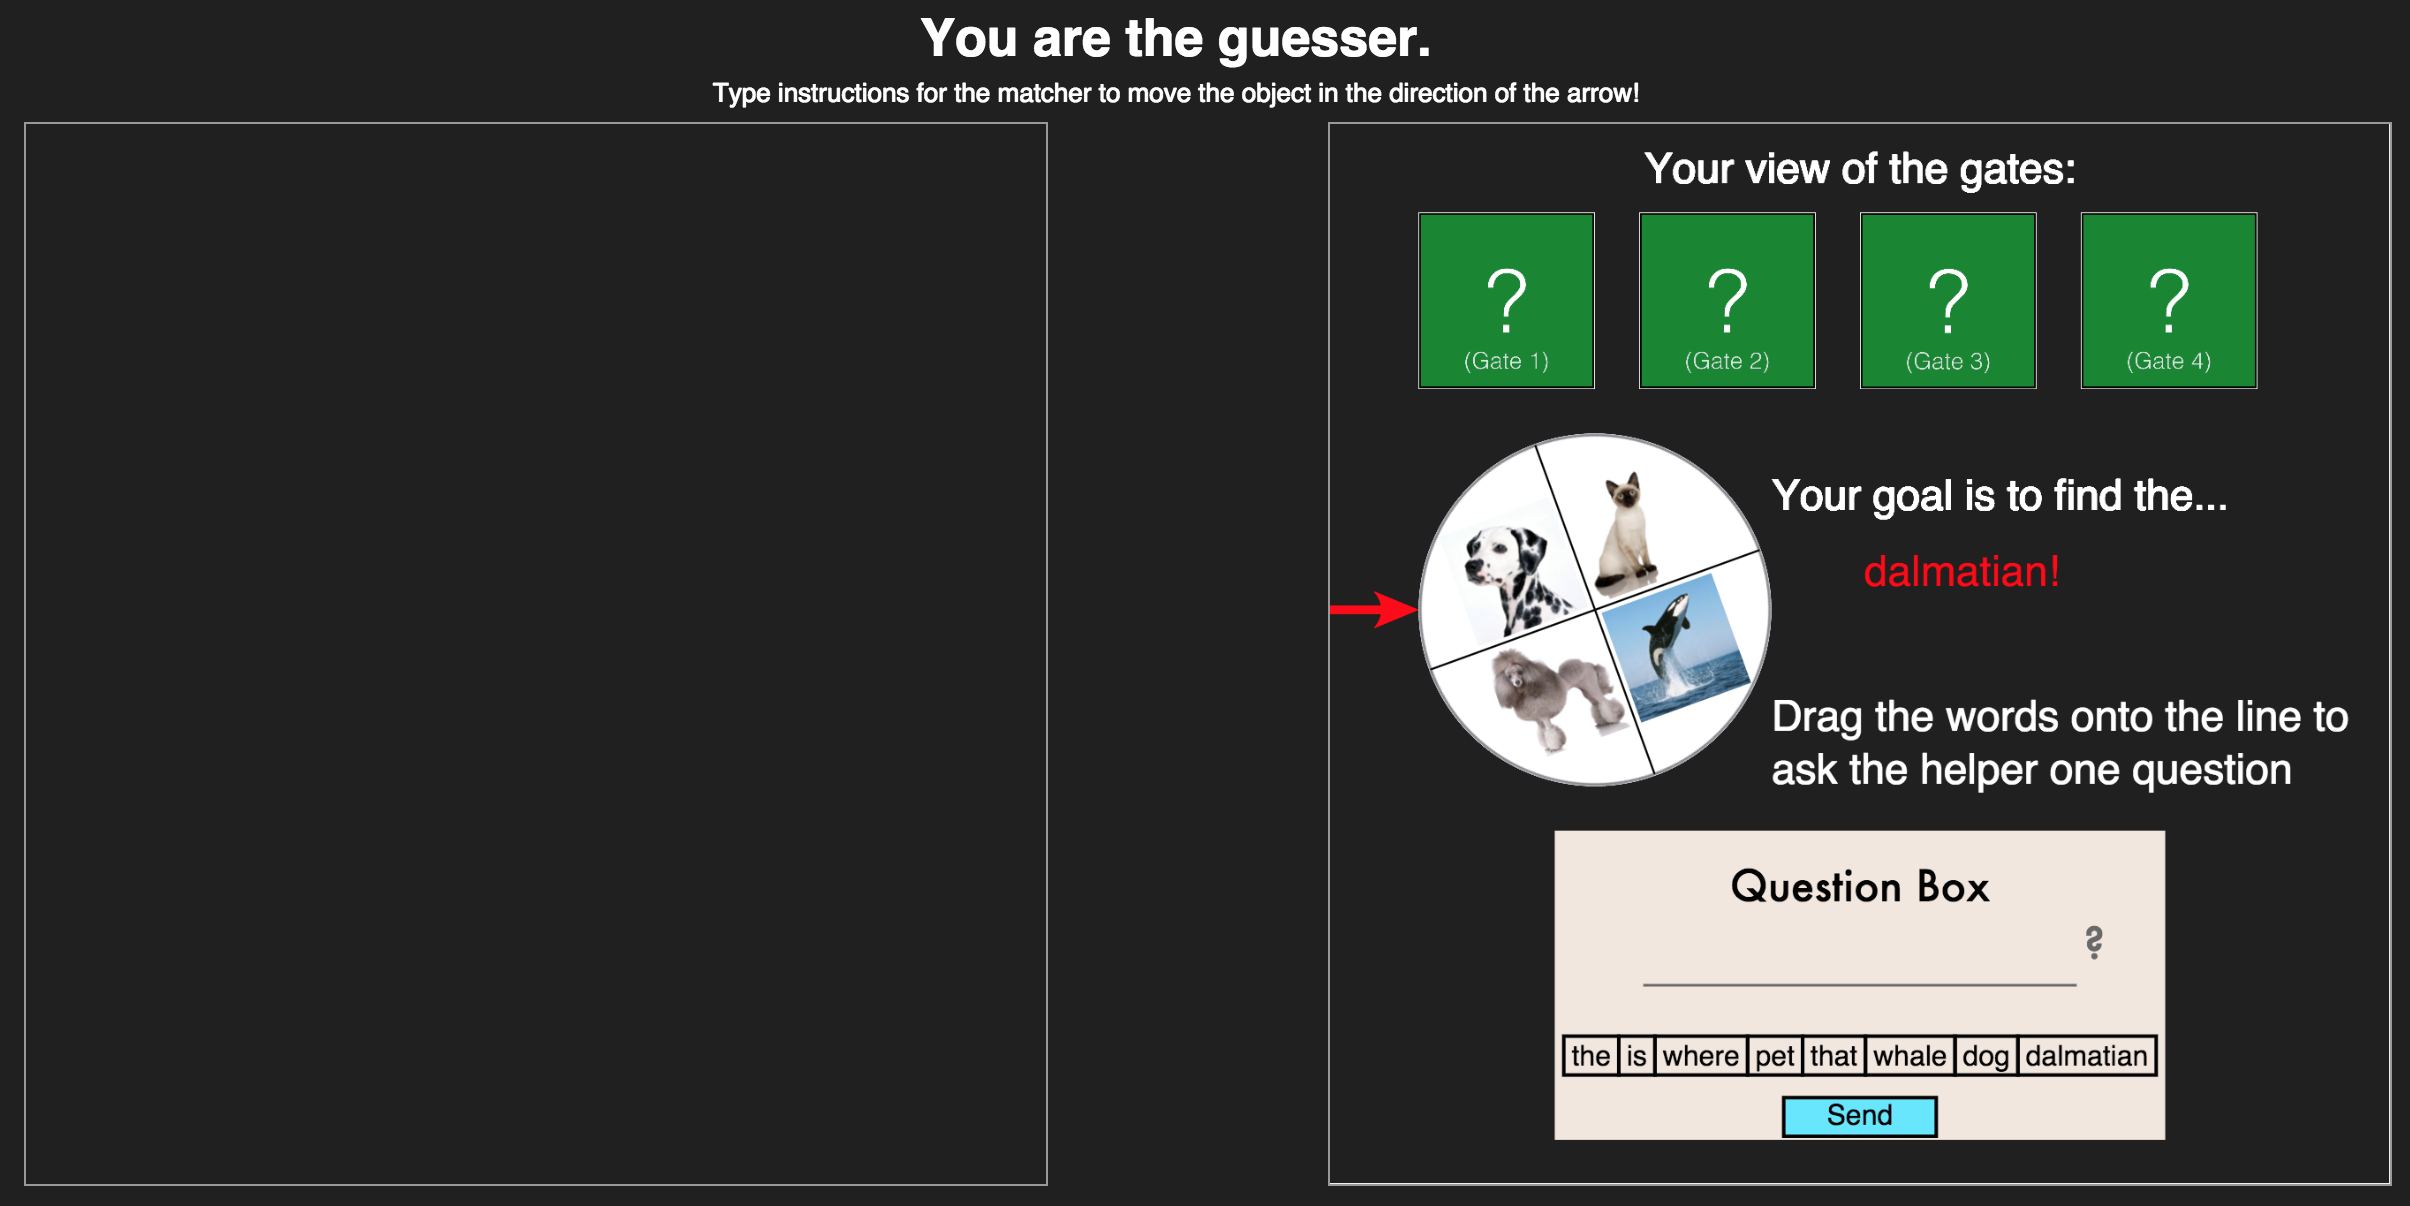
\includegraphics[scale = .3]{Exp3GuesserView}
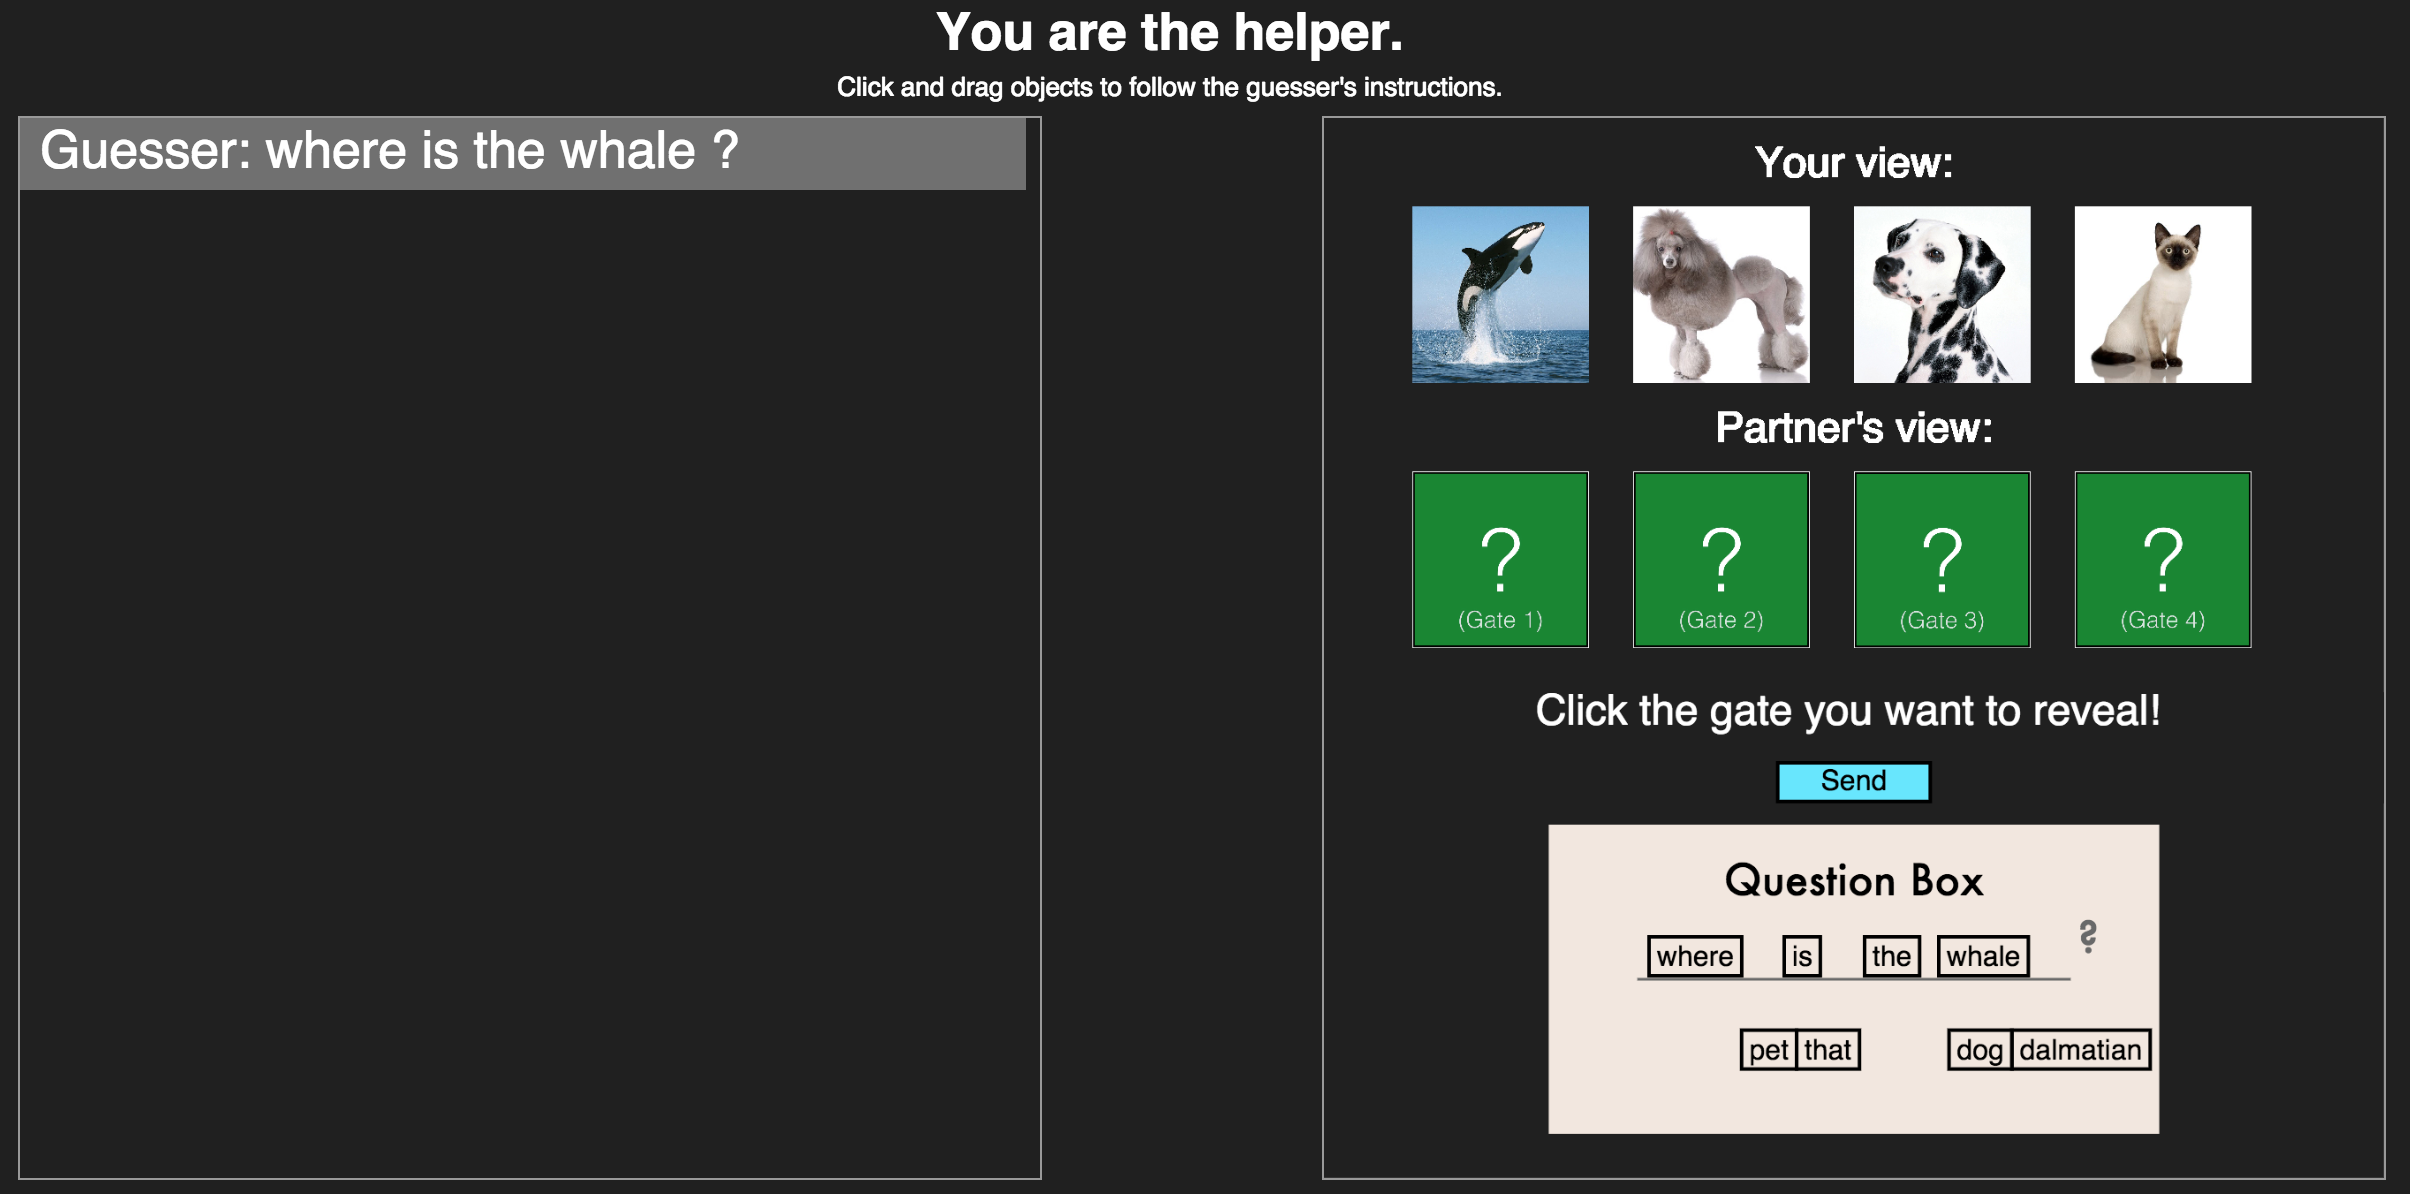
\includegraphics[scale = .3]{Exp3HelperView}
\end{center}
\caption{Exp.~3 interfaces, for the questioner (top) and answerer (bottom).}
\label{fig:exp3views}
\end{figure*}

%
%\begin{figure}[t!]
%\begin{center}
%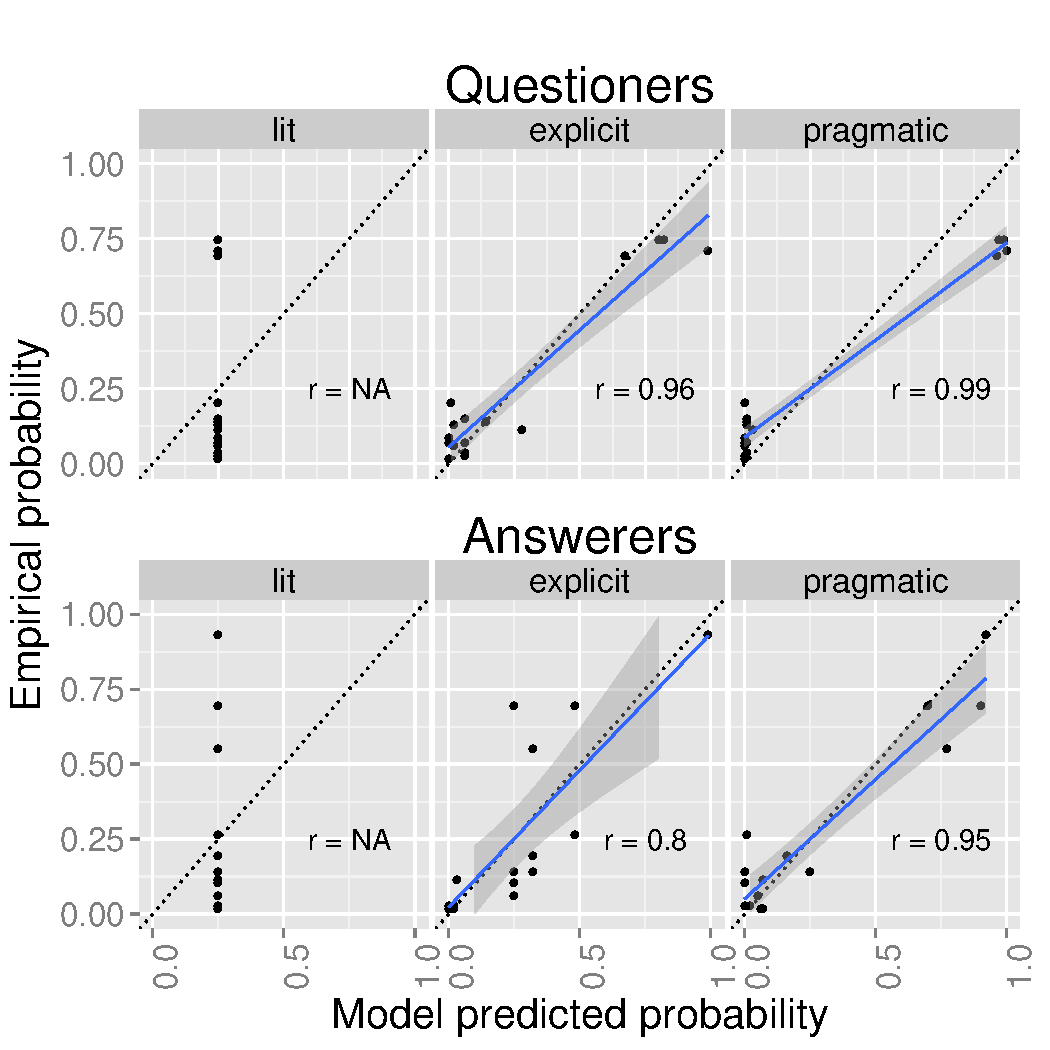
\includegraphics[scale=.75]{Exp1ModelFits.pdf}
%\end{center}
%\vspace{-.5cm}
%\caption{Full space of models, and their correlations with the data from Exp.~1. Questioner models in the first row reason about the answerers directly below them, and the pragmatic answerer reasons about the explicit questioner.}
%\label{fig:Exp1ModelSpace}
%\vspace{-.15cm}
%\end{figure}
%


In order to simultaneously test how questioners choose questions when faced with a particular goal and how answerers respond  under uncertainty about this goal, we used a guessing-game task played by two players: a questioner and an answerer. In this game, $4$ animals (a dalmatian, a poodle, a cat, and a whale) were hidden behind $4$ gates. These animals corresponded to different levels in a class hierarchy (see Fig.~\ref{fig:taskhierarchy}). The questioner received a private goal of finding one of the objects (e.g. `find the poodle'), and the answerer (but not the questioner) knew the location of each object. Before choosing a gate, the questioner asked the answerer a single question, chosen from a restricted set of options, and the answerer responded by revealing the object behind a single gate. This restriction on the question space was motivated by one of the key features of our first opening example: when the most direct question (``can I eat your food?'') is suppressed due to politeness, utterance length, complexity, or some other intervening factor, questioners must rely instead on an indirect question. 

\begin{figure*}[t!]
\begin{center}
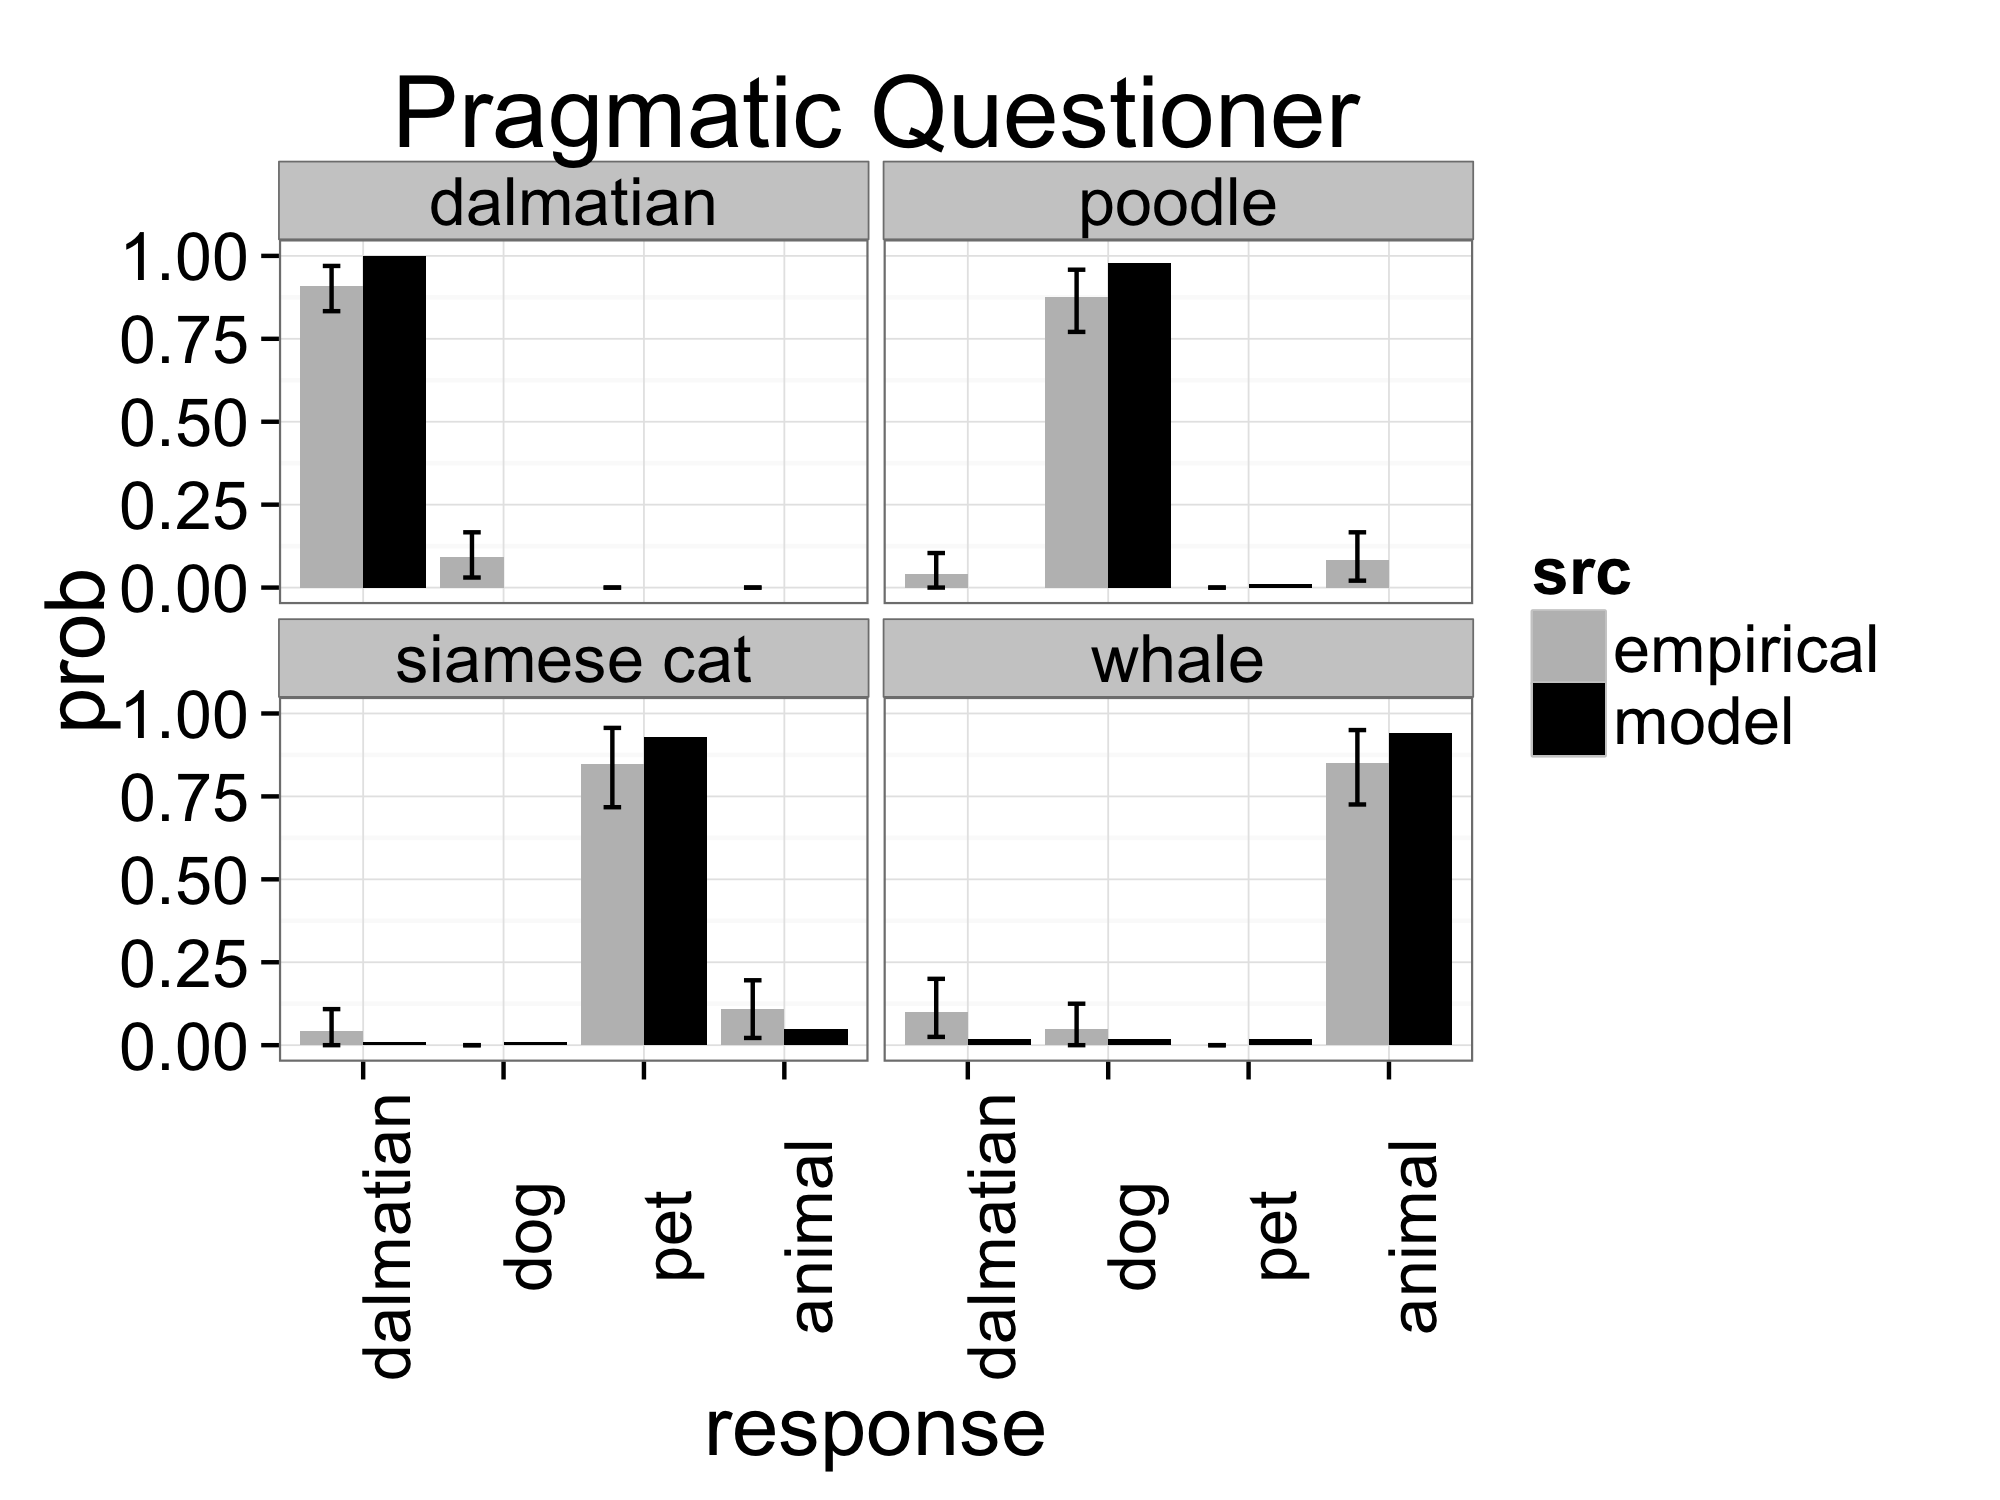
\includegraphics[scale = .11]{exp3QuestResultsPragmatic.png}
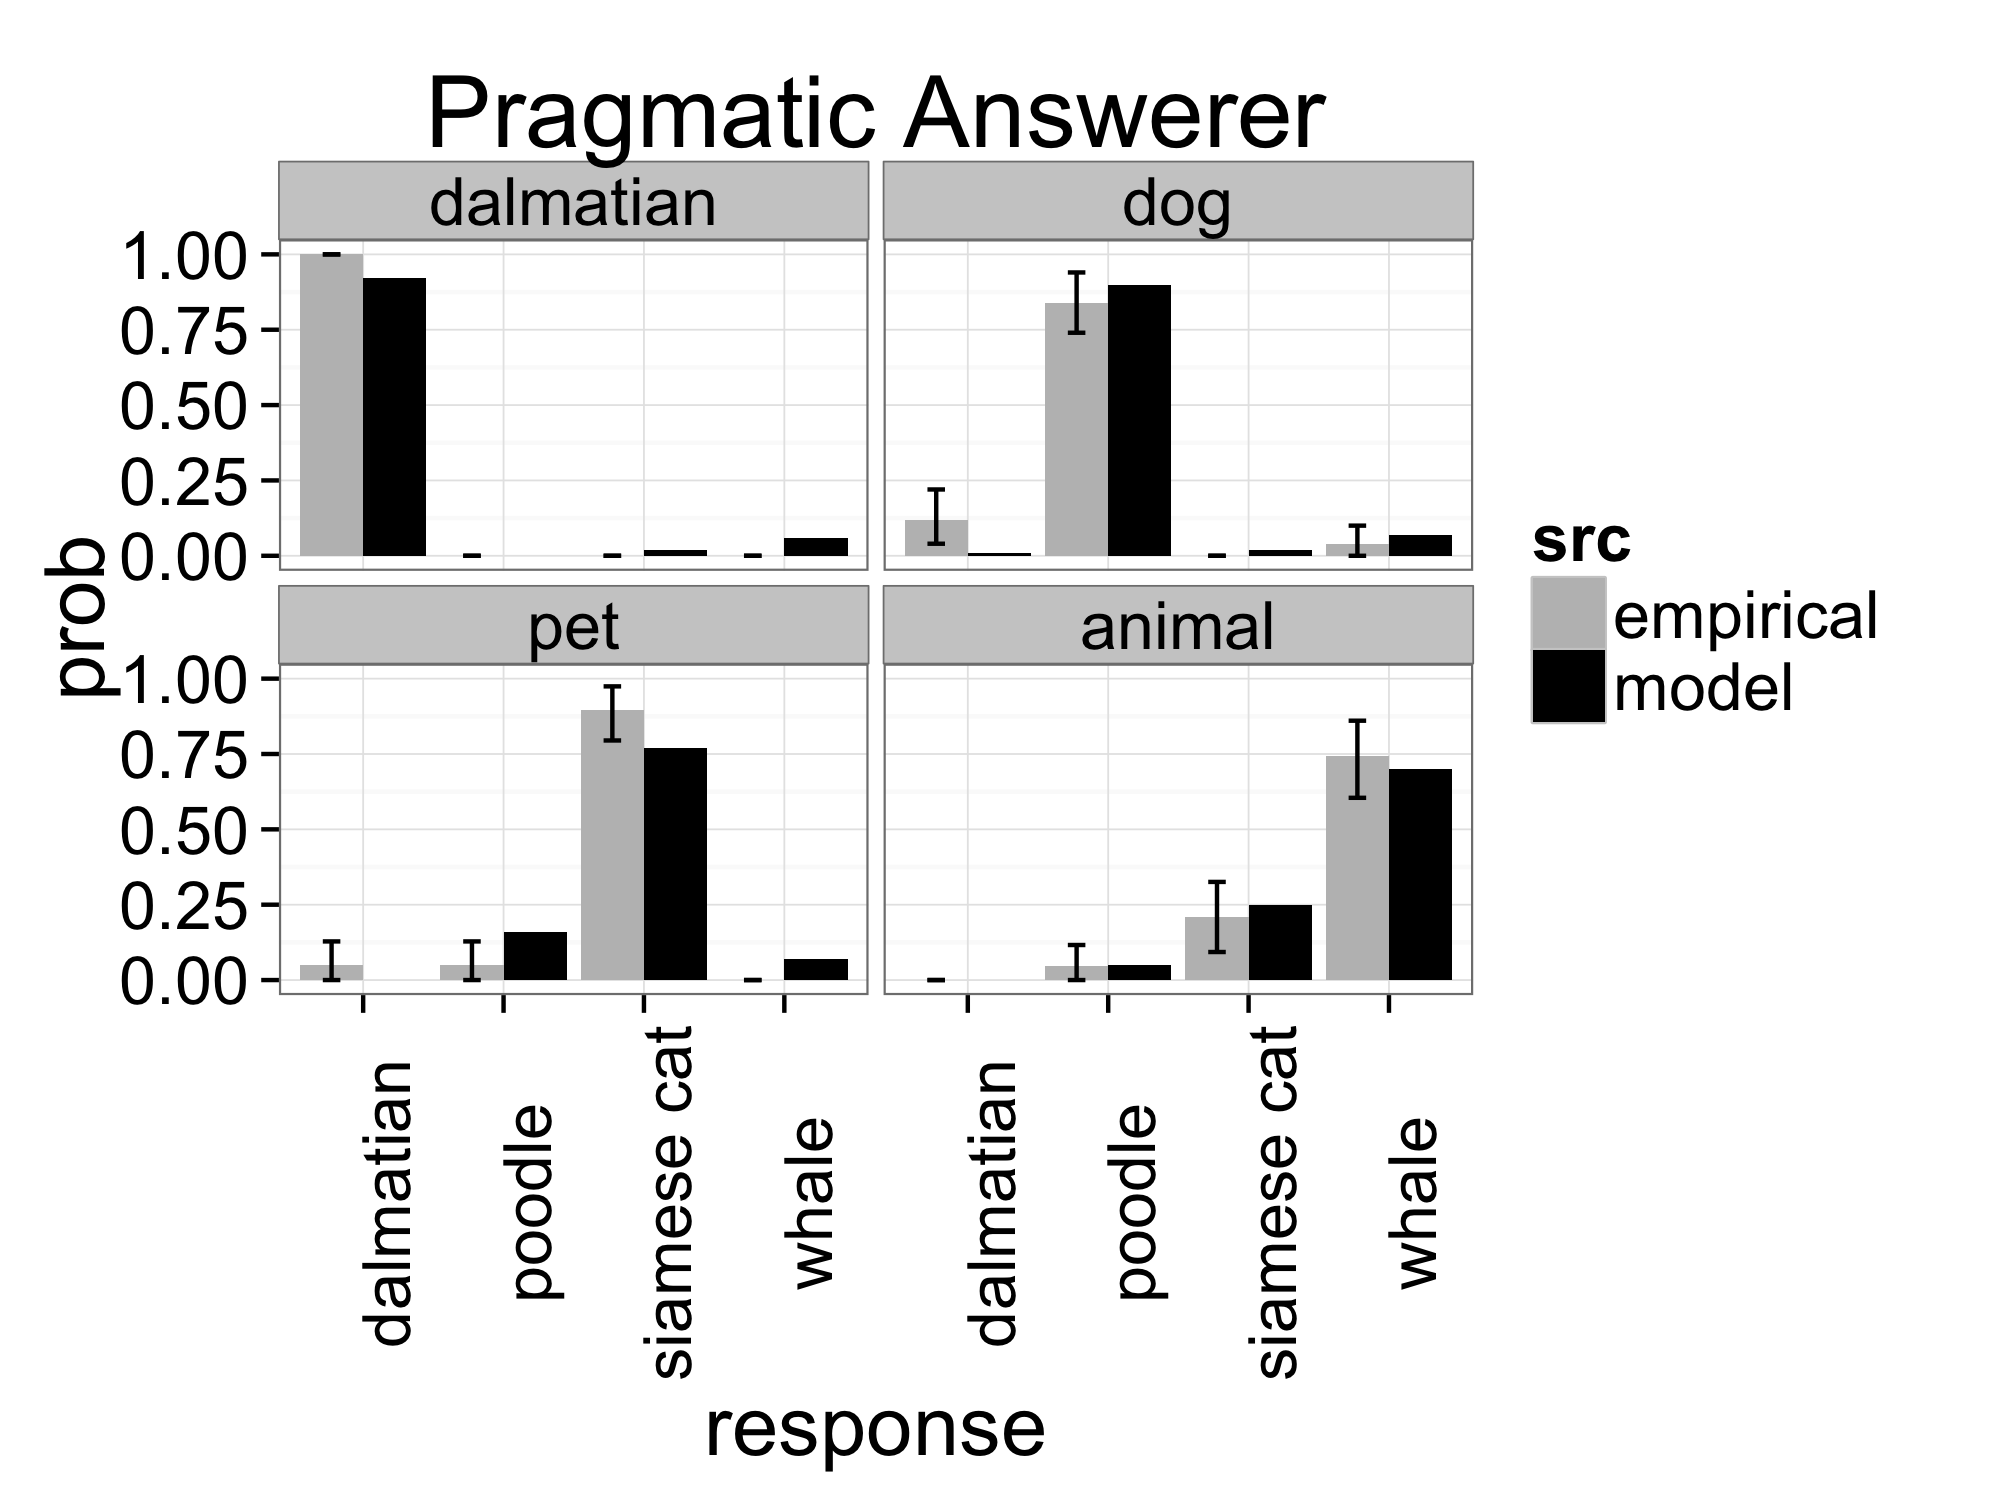
\includegraphics[scale = .11]{exp3AnsResultsPragmatic.png}
\end{center}
\caption{Exp.~1 results and model fits, for the best-performing questioner (left) and answerer (right) models. Error bars are 95\% bootstrapped confidence intervals.}
\label{fig:exp3res}
\end{figure*}
This set of restricted options was critical to distinguishing between the pragmatic and explicit variants of our model. If all questions were equally available, both our `explicit' and `pragmatic' questioner models would prefer the most direct one and would therefore be indistinguishable. To see how they make different predictions in the presence of restrictions, suppose the question `Where's the poodle?' was not available the questioner. If the questioner asked `Where's the dog?', the poodle and dalmatian would be considered equally good options by an explicit answerer because they are both dogs. However, the pragmatic answerer could reason that if the questioner was truly interested in the location of the dalmatian, he would have \emph{asked} about the dalmatian. Because he didn't, he must be interested in the other valid response that he lacks a direct question for: the poodle. Using these differing predictions, Experiment 1 was designed to distinguish between the explicit and pragmatic answerers. Similar logic allows it to also distinguish between the explicit and pragmatic questioners.

\section{Exp.~1: Interactive Questions and Answers}


\subsubsection{Participants} We recruited 50 participants
from Amazon's Mechanical Turk to participate in this task: 25 were assigned to the  questioner role and 25 to the answerer role, yielding question-answer data from 25 interactive games.

\subsubsection{Stimuli \& Procedure} In terms of our model parameters, the world space $\mathcal{W}$ was the set of $4! = 24$ possible assignments of four objects to four gates. The goal space $\mathcal{G}$ was the set of four objects that the questioner could be trying to find: `dalmatian,' `poodle,' `siamese cat,' and `whale.' These objects correspond to the leaves of the tree in Fig.~\ref{fig:taskhierarchy}. The answer space $\mathcal{A}$ was the set of four gates that the answerer could  reveal. The restricted question space $\mathcal{Q}$ contained the set of highlighted nodes in the taxonomy: `dalmatian?', `dog?', `pet?', and `animal?' (see Figure \ref{fig:taskhierarchy}). 

\begin{figure*}[t!]
\begin{center}
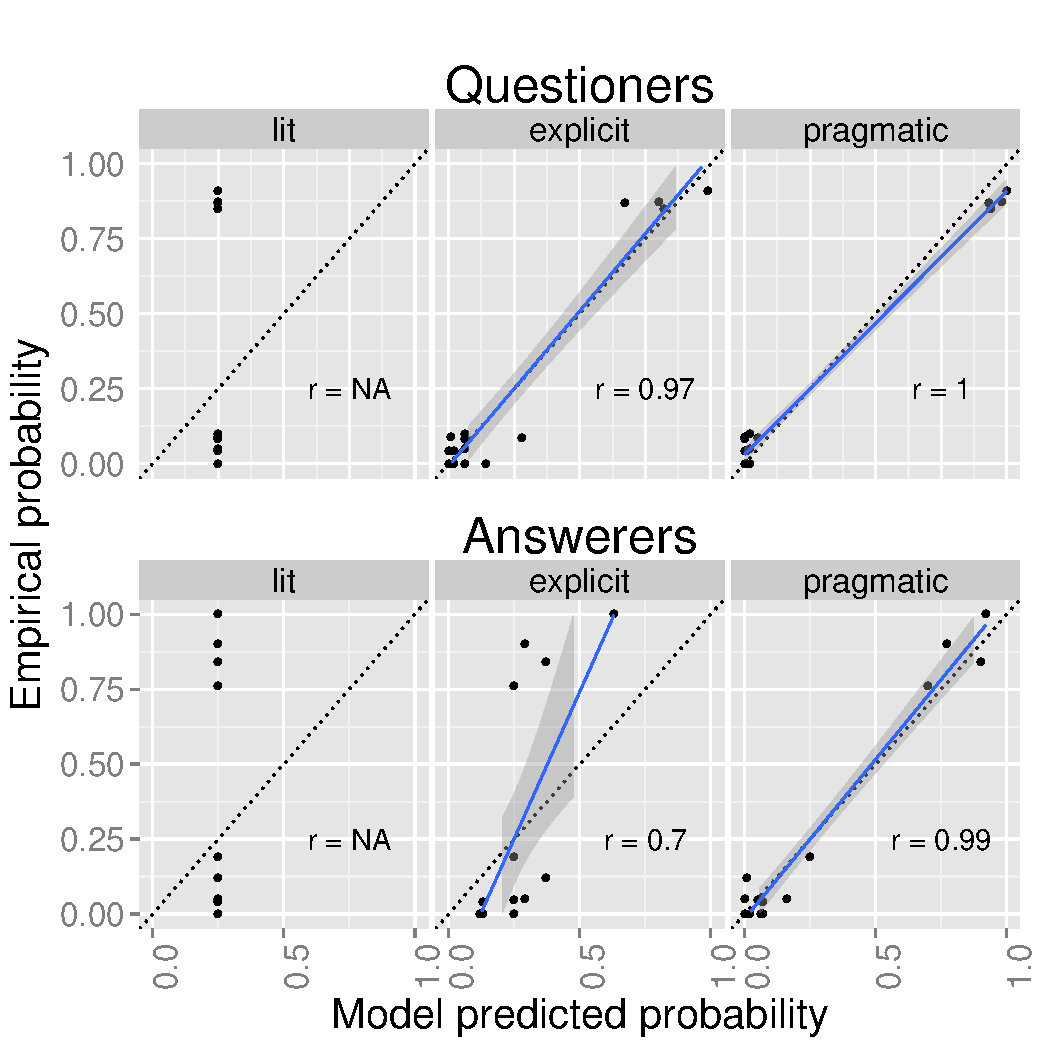
\includegraphics[scale=.75]{Exp3ModelFits.pdf}
\end{center}
\caption{Full space of models, and their correlations with the data from Exp.~1. Questioner models in the first row reason about the answerers directly below them, and the pragmatic answerer reasons about the explicit questioner.}
\label{fig:Exp3ModelSpace}
\end{figure*}

The procedure was designed to accommodate real-time player-to-player interaction following \citeA{Hawkins14_RealTimeWebExperiments}. All players passed a short quiz on the game instructions and were immediately redirected to the game interface: the first player to join was assigned to be a ``questioner'' (which we called a ``guesser'' in the cover story) and told to wait until a second player was available. Once another player joined, they were assigned to be an ``answerer'' (or ``helper'') and the game began. 

The questioner and answerer interfaces are displayed in Figure \ref{fig:exp3views}. Chat messages were printed on the left side of the screen, and players used the right side as a workspace to view goals, ask questions, and respond with answers. At the beginning of each trial, the wheel on the questioner's screen (Figure \ref{fig:exp3views}, top) would spin and select one of the four goals at random. The questioner then clicked and dragged words onto the line in the ``Question box'' to ask a question to help them find this goal. The answerer saw these words being dragged in real time. Once the questioner clicked the `send' button, the resulting question appeared in the chat log and control was passed to the answerer, who clicked on one of the four gates to automatically send a response containing the location of the chosen object (e.g. ``The whale is behind gate 3.'') Finally, the questioner was asked to guess which gate they believed the goal object was behind. 

Each participant provided responses for four trials, where object locations were shuffled and a new goal was randomly selected for each trial. Thus, questioners could be given the same goal on multiple trials, preventing `process of elimination' reasoning about what the goal may be.

\subsubsection{Results}
%\red{check for effect of Q/A block order.}
Results for the questioner role are shown alongside model predictions in Fig.~\ref{fig:exp3res} (left). We find that questioners systematically prefer to ask different questions given different goals, even as those questions become more indirect. $\chi^2$ tests over each of the four response distributions show a significant divergence from uniform. Questioners preferentially ask about the `dalmatian' given the  dalmatian goal, ${\chi^2(3) = 77}, {p < .001}$, about the `dog' given the poodle goal, ${\chi^2(3) = 50}, {p <.001}$, about the `pet' given the cat goal, ${\chi^2(3) = 47},  {p <.001}$, and about the `animal' when given the whale goal, ${\chi^2(3) = 39}, {p <.001}$. Note that there was a high level of agreement between participants on the best question to ask: questioner responses were not particularly graded.

Results for the answerer role are shown in Fig.~\ref{fig:exp3res} (right). Answerers are highly sensitive to the constraints of the questioner, giving information about the dalmatian when asked about a `dalmatian', ${\chi^2(3) = 102}, {p <.001}$, about the poodle when asked about a `dog', ${\chi^2(3) = 47}, {p <.001}$, about the cat when asked about a `pet', ${\chi^2(3) = 45}, {p<.001}$, and about the whale when asked about an `animal', ${\chi^2(3) = 31}, {p < .001}$. In the next section, we compare these results to the predictions of our family of models (Fig. \ref{fig:Exp3ModelSpace}). 

\subsubsection{Model comparison}

Each model was run with uniform prior probability over worlds, goals, questions, and answers, and with equal cost for all utterances. The goal projection for goal object $o$ is given by $$g_o(w) = \textrm{loc}(o,w)$$ where $\textrm{loc(o,w)}$ is a simple function looking up the location of object $o$ in world $w$. 

The explicit meaning of the question ``Where's the $x$?'' maps a world $w$ to the location of the salient object of type $x$. This implements the standard formal semantics of \emph{the}: the denotation of a noun phrase containing a definite article is only defined if there is a unique, salient object that the noun picks out in the world. Pragmatically, the use of a definite article \emph{presupposes} the salience of some object. Thus our explicit QUD is: 
$$\textrm{\den{Where is the N?}} = q_{N}(w) = \textrm{loc}(s_N,w)$$ where $s_N$ is the salient object of category $N$. 

Because the answerer does not know \emph{a priori} which object is the salient one, they draw an object from a saliency distribution, given the category in the noun phrase $s_N \sim \mathcal{S}(o | N)$. This distribution may depend on typicality judgements \cite{Rosch75}, world knowledge about what labels people tend to use to refer to an object, and so on. For current purposes, we take the saliency prior to be uniform over all objects that are within a category (e.g. over all leaves of the subtree beneath the given label; see Fig. \ref{fig:taskhierarchy}). 

Note that other variations of the question that were not used in our experiment, such as ``Where \emph{are} the animal\emph{s}?'', would be given different semantics (in this case projecting a world to the set of all locations occupied by animals rather than the single location of the salient animal). The goal of our study is not to test these semantic theories, but to test models of social reasoning that gives rise to question-answer pragmatics.

 For each model, a single optimality parameter, which applied to all agents as described above, was fit to maximize correlation with the data. We can immediately rule out both the literal answerer and literal questioner as they predict a uniform distribution of responses over the four questions and answers. The two remaining questioner models make roughly the same predictions for this task:
we found a model-data correlation of $r = 0.971$ for the explicit questioner and correlation of $r = 0.996$ for the pragmatic questioner. The difference between these correlations is statistically significant, accounting for their shared dependence on the empirical data \cite[Zou's 95\% confidence interval \textrm{= [-0.079, -0.009]}]{DiedenhofenMusch14_cocor}. However, they make nearly identical qualitative predictions; the pragmatic questioner model's predictions for each response distribution are shown in Fig.~\ref{fig:exp3res} (left). 

The pragmatic answerer provides a much better fit to the data than the explicit answerer: we find a model-data correlation of $r = 0.7$ for the explicit answerer and $r = 0.99$ for the pragmatic answerer.  Taking into account the fact that these correlations are dependent and overlapping on the same empirical data, we find that the pragmatic answerer correlation is significantly larger than the explicit answerer correlation (Zou's confidence interval $= [-0.676, -0.107]$). 


\subsubsection{Discussion}

%We replicated the results of experiment 1 in a real-time, interactive setting. Again, we found that both explicit and pragmatic questioner models provide an excellent fit to questioner behavior, and that the pragmatic answerer accounts for the data significantly better than the explicit answerer both quantitatively and qualitatively. In addition, the full, interactive game was designed to be more natural and less confusing to participants than the drop-down menu design from experiments 1 and 2. Because players received constant feedback from their partner, this task was framed as inherently social, and because answerers watched as questioners moved words to form questions, there was a convincing mechanism for people to believe they were playing with another human. This addresses some concerns raised with experiments 1 and 2. 
Only the pragmatic answerer can account for essential qualitative features of the response data. For example, the explicit answerer predicts that participants will be equally likely to show the `dalmatian,' `poodle,' and `cat' when asked about a pet. Instead, the data show a significant preference for revealing the cat, leaving `dalmatian' and `poodle' at the same level as the other alternative. The pragmatic answerer correctly predicts this pattern  (see Fig.~\ref{fig:exp3res} (right)). Even more dramatically, the explicit answerer predicts a uniform distribution over responses to the `animal?' question. %(since all four responses denote animals)
Contrary to these predictions, we found that answerers overwhelmingly preferred the response ``whale'' to the other three responses, and this response distribution was significantly different from uniform. 

While this model comparison is a strong result, we also identified four major shortcomings of Experiment 1. First, our data are much more equivocal with respect to distinguishing between the explicit and pragmatic \emph{questioner} models. The two models did not make significantly different predictions for this experiment (and both are sufficient to account for the data). 

Second, the stimuli in Experiment 1 all derived from a single hierarchy containing animal categories. This provided only 16 points of comparison between our models and empirical data. We would like to show that our model generalizes to different hierarchy structures and different category domains such as plants, places, and artifacts. 

Third, at least in the case of our Experiment 1 hierarchy, there exists a simple, heuristic strategy that produces the same pattern of responses as our model without requiring any social inference. Suppose questioners saw their goal on a given trial and ruled out labels that do not apply (e.g. a `cat' is neither a `dalmatian' nor a `dog'), then picked the most specific of the remaining labels (`pet' picks out a smaller set of objects than `animal'). Whether through use of this heuristic strategy or pragmatic inference (as our model suggests), questioners strongly converged on a single mapping from goals to question utterances. 

Finally, because there was overwhelming agreement among participants on the appropriate question to ask and the appropriate answer to give, our response probabilities are clumped at the ends of the scale. Thus, while there is an excellent quantitative fit between our model and the data, we're essentially fitting endpoints. We would like to collect more graded judgements between these endpoints, where our model predicts that participants will disagree.
 
In response to these shortcomings, we designed a follow-up experiment, which tests the generality of our model by expanding the stimulus set to encompass multiple stimulus domains and multiple hierarchy structures designed to elicit graded judgements. In particular, this addresses the concern that the behavioral patterns we have been modeling are specific to the set of four animals or the tree-like hierarchy in which they were embedded. We also took care to include one simple but critical hierarchy structure where (1) the explicit and pragmatic questioner models make different predictions and (2) the heuristic strategy cannot mimic these predictions. 
	\begin{figure*}[t!]
\begin{center}
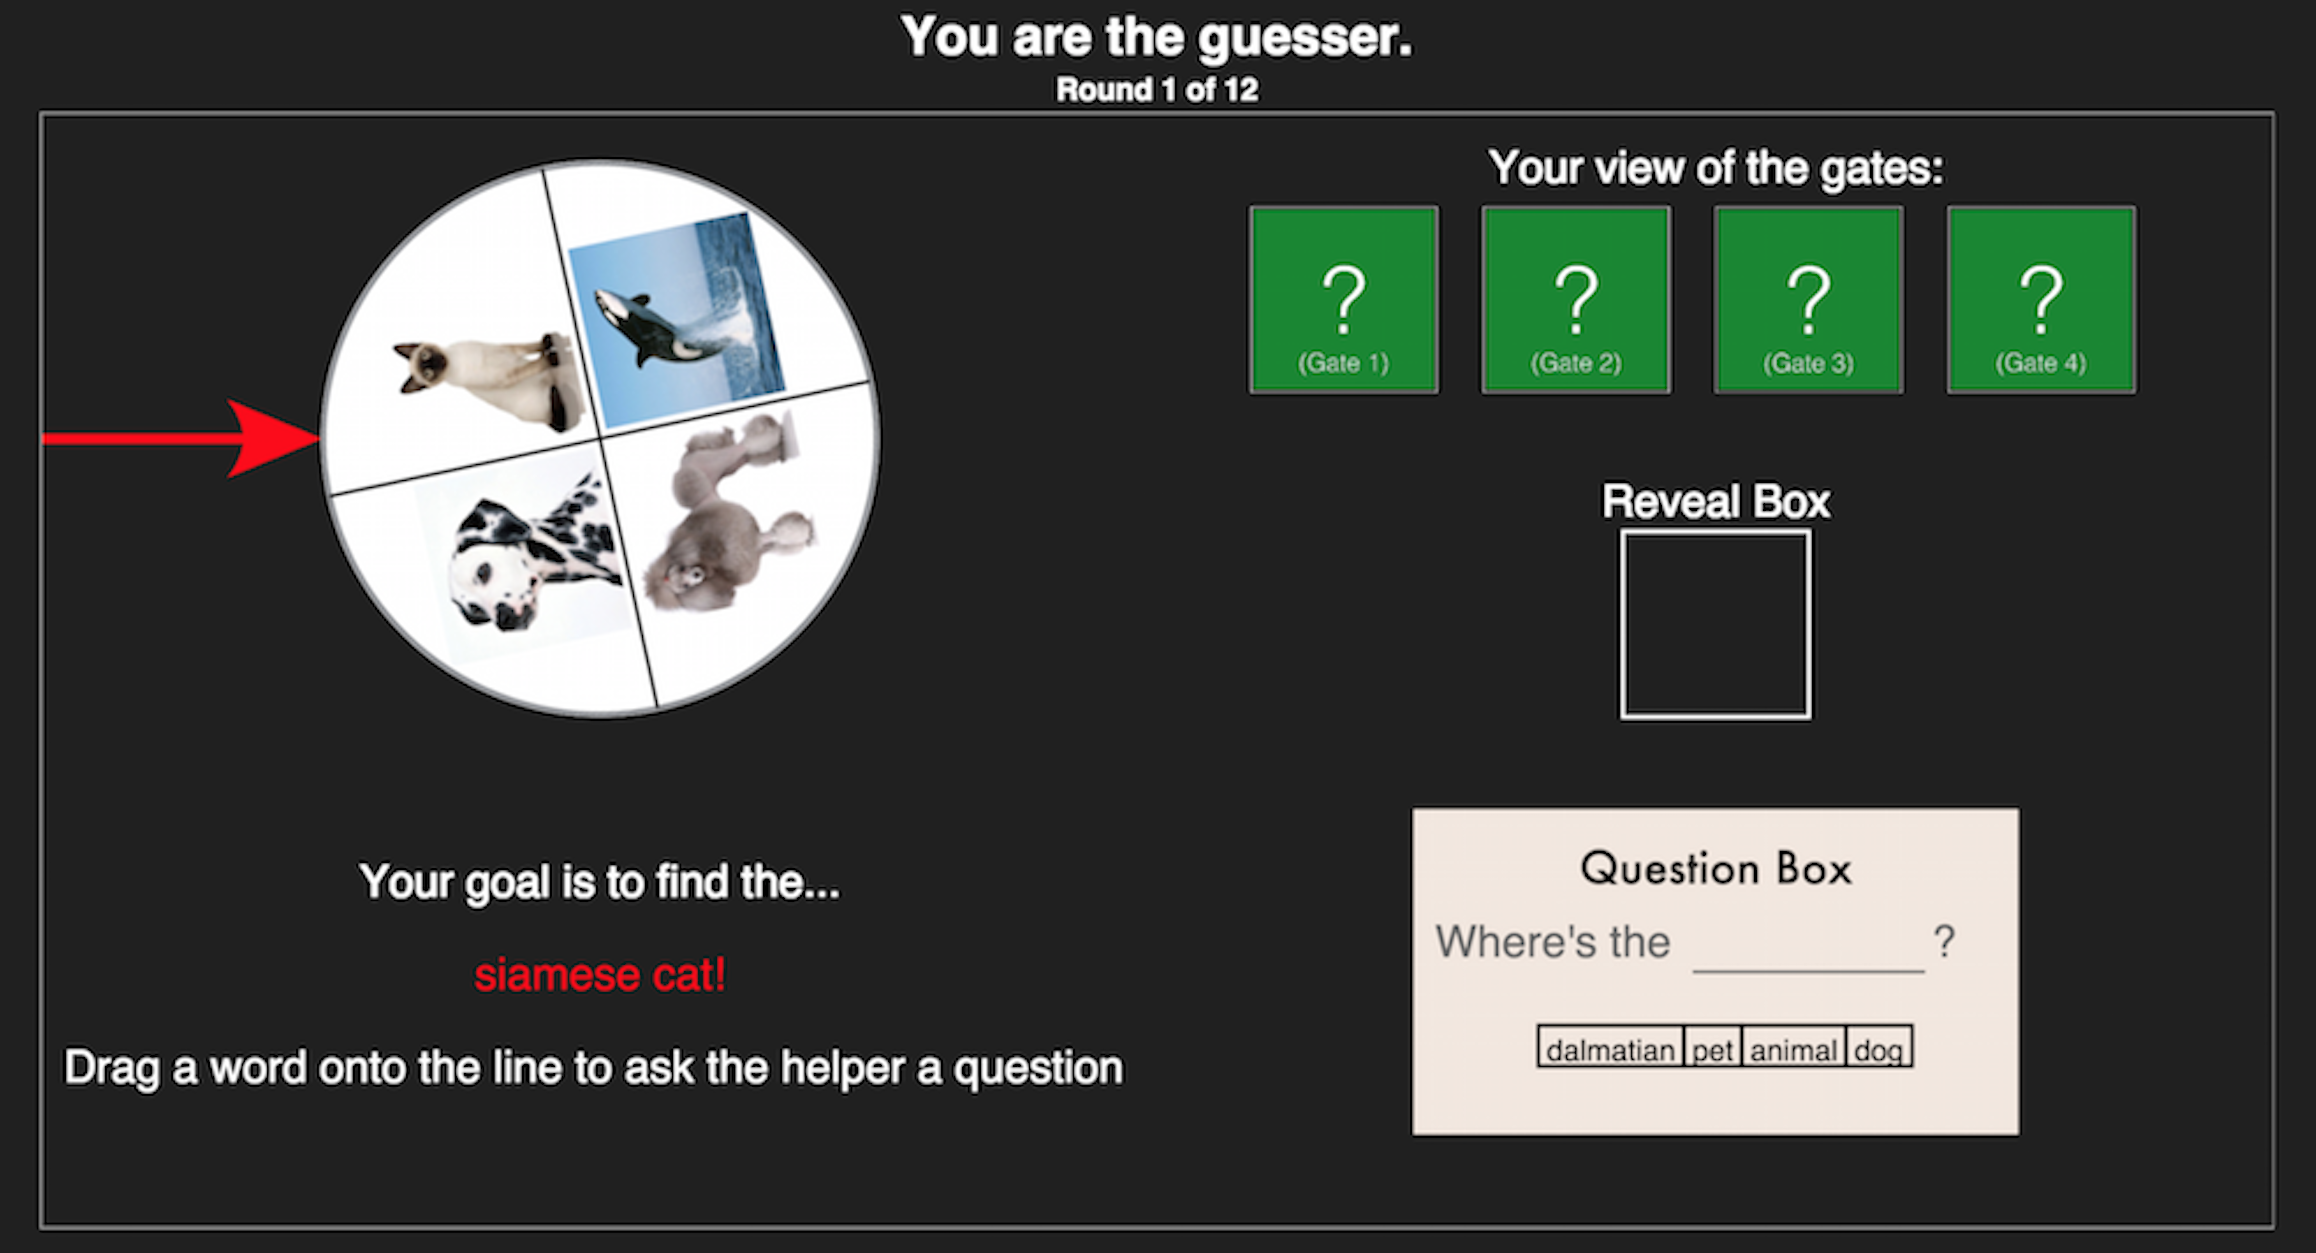
\includegraphics[scale = .3]{Exp4GuesserViewStart}
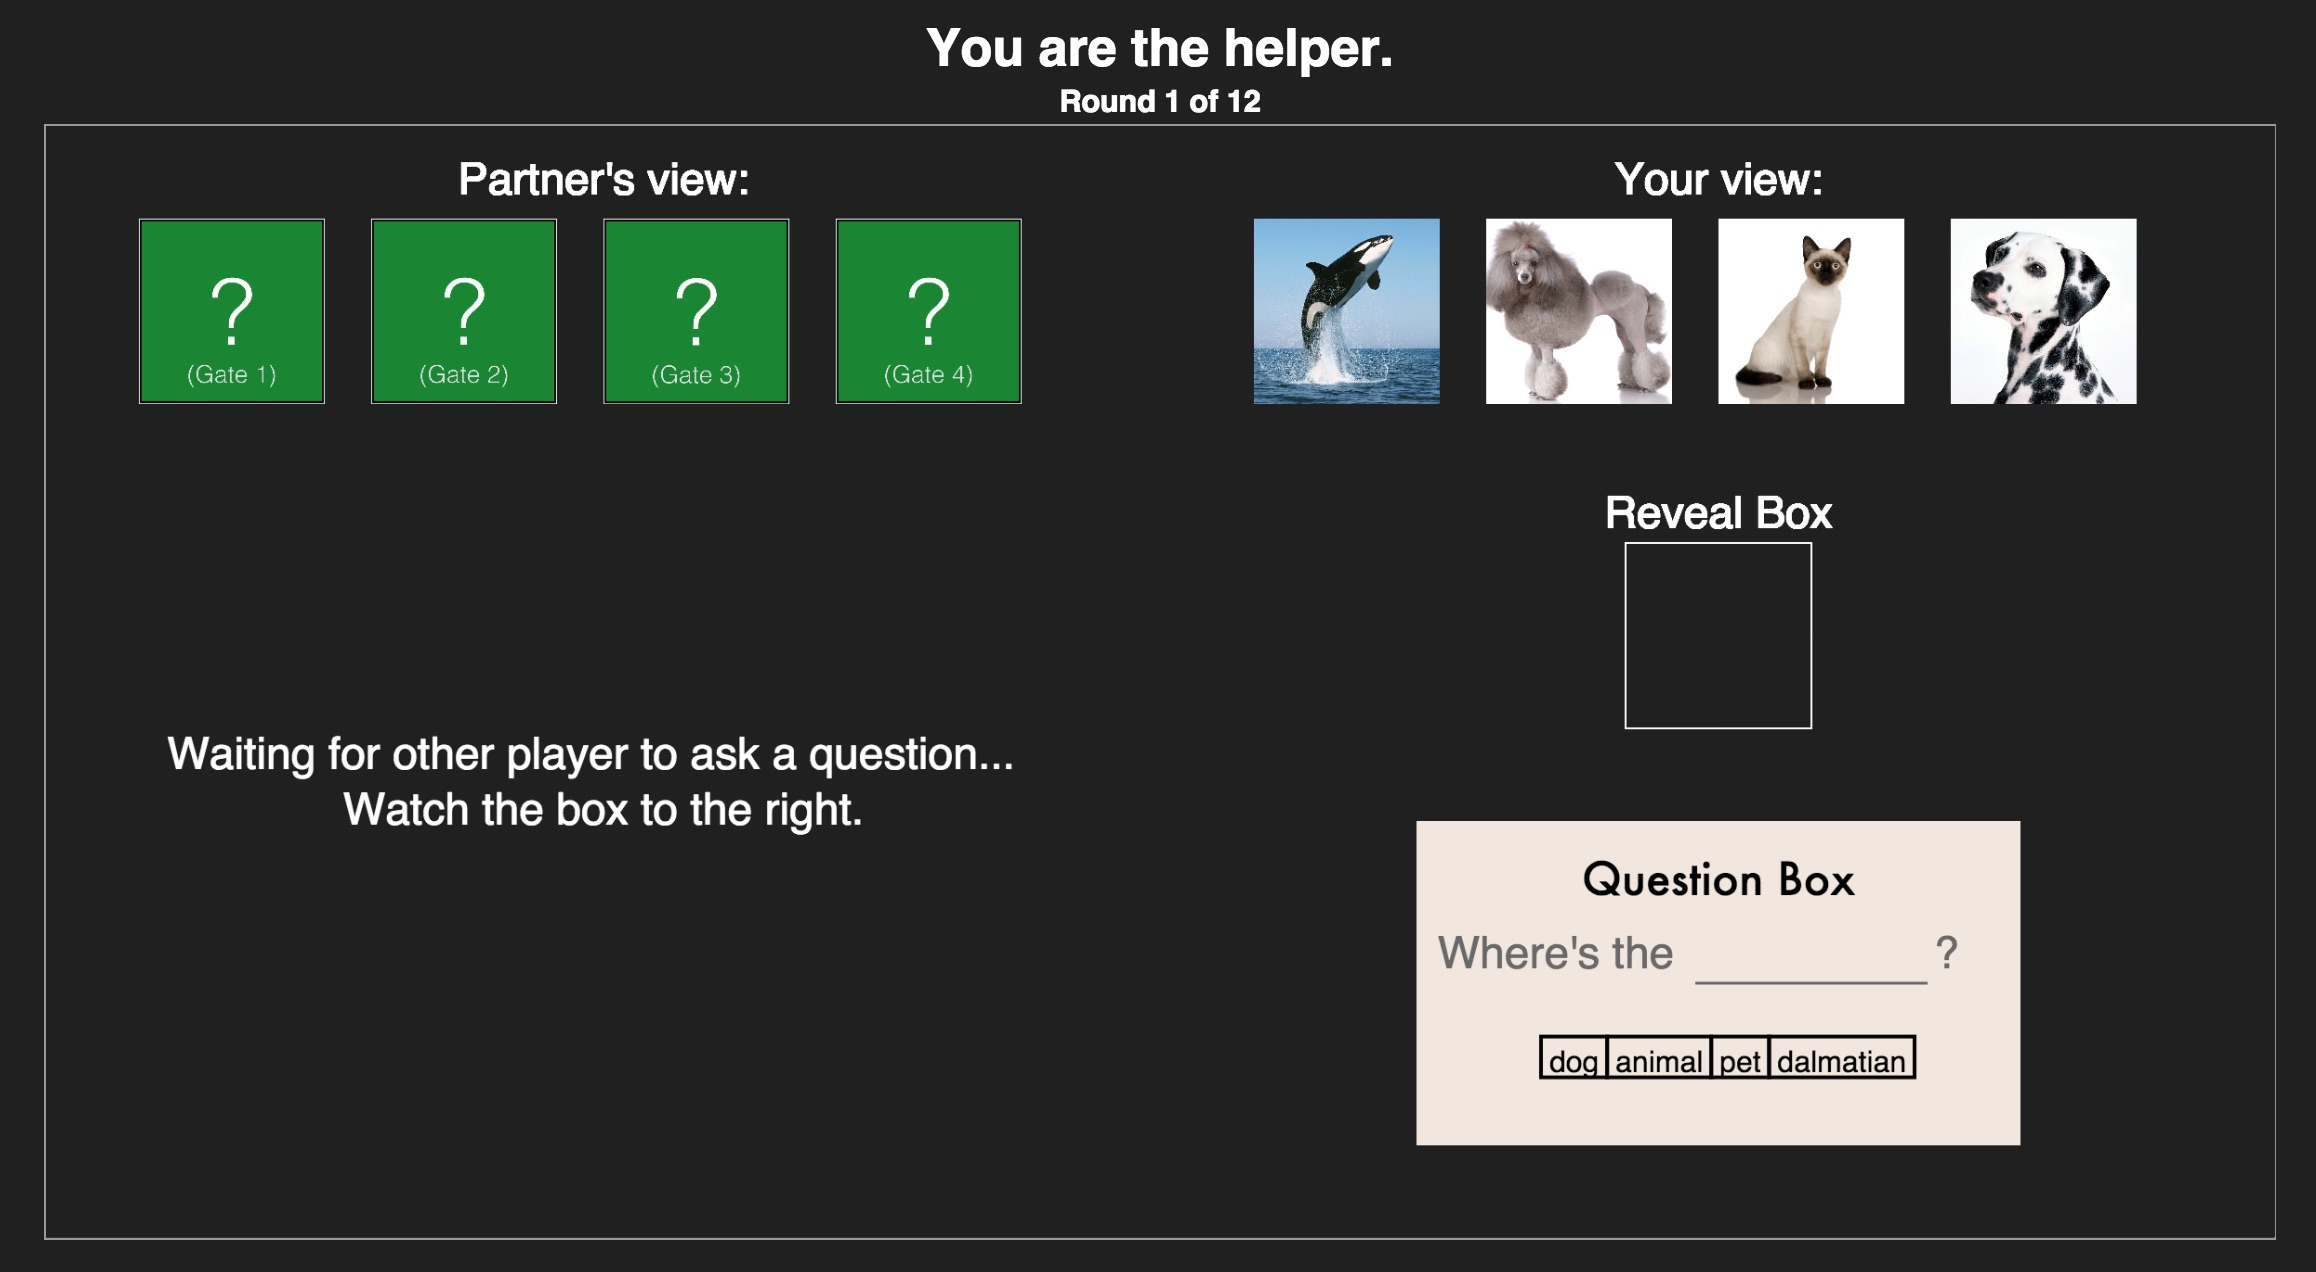
\includegraphics[scale = .15]{Exp4HelperViewStart}
\end{center}
\caption{Exp.~2 interfaces, for the questioner (top) and answerer (bottom).}
\label{fig:exp4views}
\end{figure*}
\section{Exp.~2: Generalizing Predictions}

\subsubsection{Participants} We recruited 199 participants
from Amazon's Mechanical Turk to participate in this task. Fifty participants were excluded due to a server crash that terminated the task before completion. Two additional participants were excluded because they were not non-native English speakers. This left 74 unique completed games.


\subsubsection{Stimuli \& Procedure} A set of twelve items were created by crossing four domains (animals, plants, places, and artifacts) with three hierarchy structures (``branching'', ``overlapping'', and ``equivocal''; see Figure \ref{fig:hierarchyStructures}). For each item, there was a set of four goal objects in $\mathcal{G}$, which appeared on the wheel for the questioners, four question labels in $\mathcal{Q}$ that the questioner could use to ask about their assigned goal, and four answers in $\mathcal{A}$ corresponding to the four items in $\mathcal{G}$ that appear on the wheel.\footnote{A document containing these mappings for all items, as well as their hierarchical relationships, is available online at \url{https://github.com/hawkrobe/Q\_and\_A/blob/master/MultiExperiment2/stimuliLabels.pdf}} 

	\begin{figure*}[t!]
\begin{center}
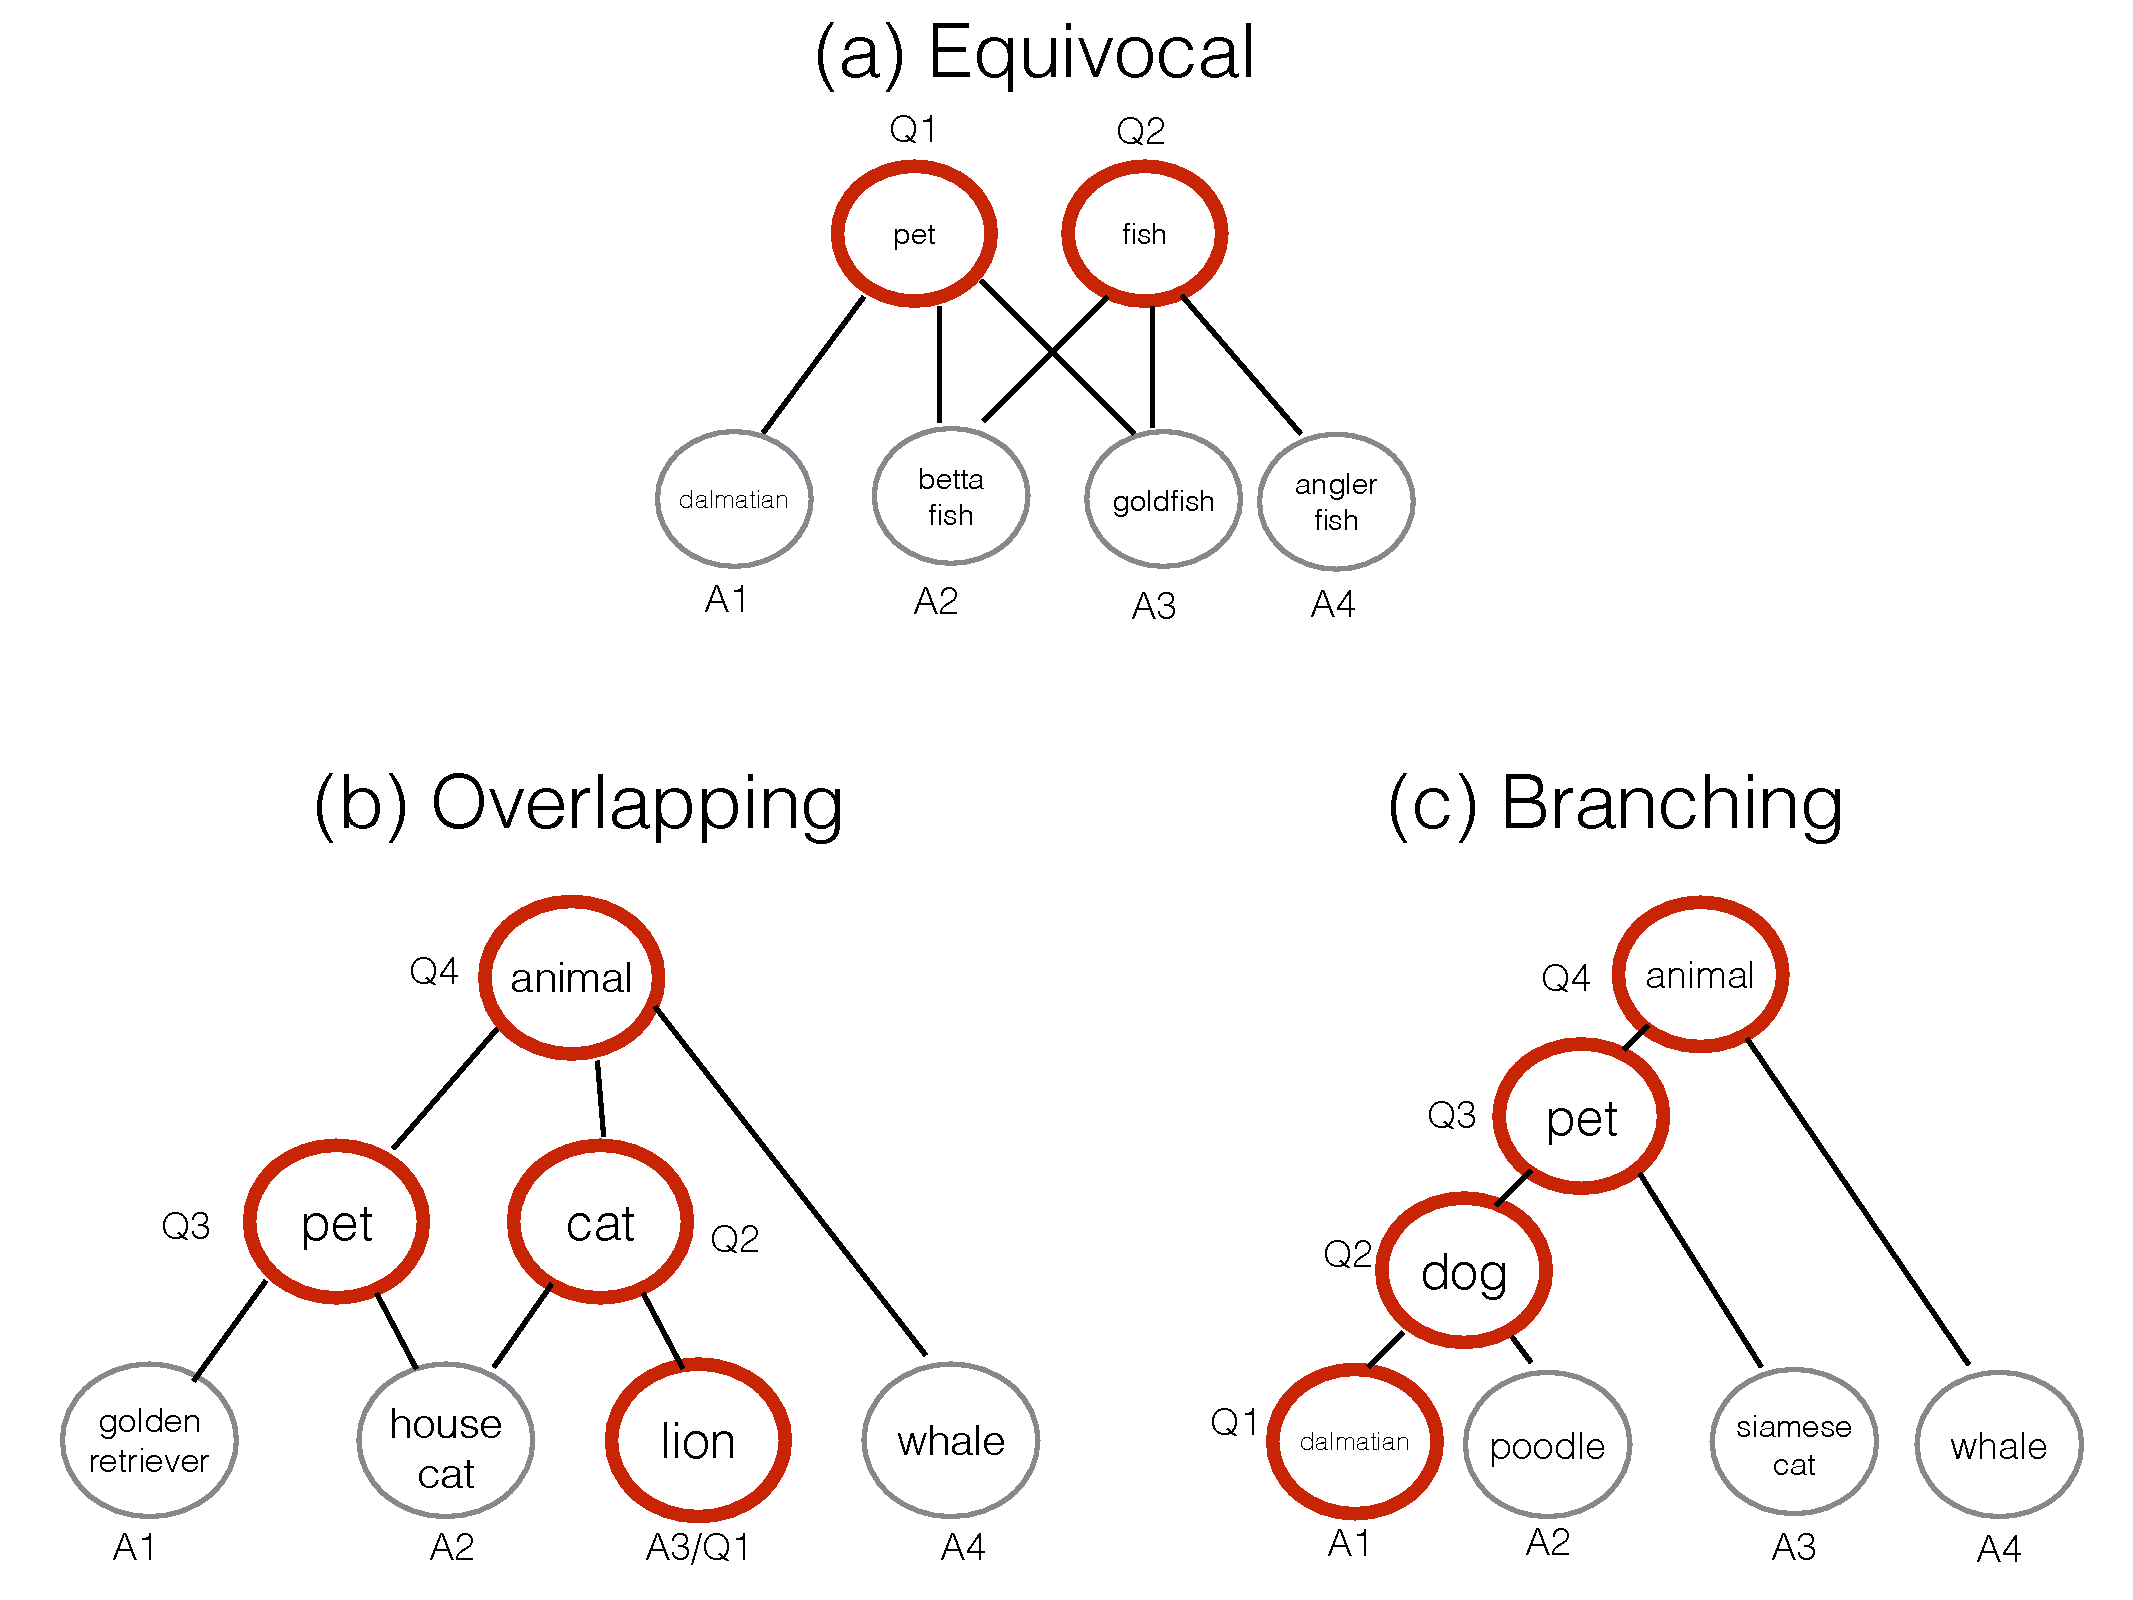
\includegraphics[scale = .3]{hierarchyStructureExamples}
\end{center}
\caption{Example of each type of hierarchy used in Experiment 2. The bottom row served as the answer space, and the labels in the questioner space highlighted in red. }
\label{fig:hierarchyStructures}
\end{figure*}
\begin{table*}[t!]
\centering
\begin{tabular}{ p{1.5cm} | r | r | r | r |||||| r | r | r | r |}
& \multicolumn{4}{c||||||}{Questioners} & \multicolumn{4}{c}{Answerers} \\
&             animal &     place &     plant &  artifact &            animal &     place &     plant &  artifact \\
\hline
animal &   1.00 &  0.91 & 0.94 & 0.94 & 1.00 & 0.78 & 0.92 &  0.97 \\
\hline
place &    0.91 &  1.00 & 0.96 & 0.95 & 0.78 & 1.00 &  0.78 & 0.78 \\
\hline
plant &    0.94 & 0.96 & 1.00 & 0.97 & 0.92  & 0.78 &  1.00 & 0.91\\
\hline
artifact & 0.94 & 0.95 & 0.97 & 1.00 & 0.97 & 0.78 &  0.91 & 1.00\\
\end{tabular}
\\[1.5pt]
\caption{Inter-domain correlations in Experiment 4} 
\label{table:experiment4correlations}
\end{table*}
The procedure was the same as Experiment 1 with two major modifications. First, we addressed an asymmetry in the task: the answerer watched the questioner move words, but the questioner only saw template text responses in response. In an exit survey, we found that answerers were more likely to believe they were playing with a  human partner than questioners. To bring questioner and answerer expectations closer together, we changed the mechanism by which the answerer responds. Instead of clicking on a gate and then clicking the `send' button, we supplied a ``Reveal Box.'' When the answerer was ready to reveal a gate, they would simply click and drag the object they wanted to reveal into this box. The questioner watched as the outline of the gate moved, in real time, and saw the image as soon as the answerer dropped it in the box. 

Second, we noticed that some players began exploiting the freedom of the ``question box'' drag-and-drop procedure after playing several rounds. On difficult items, especially those in the equivocal hierarchy where our model predicts no preferred question for certain goals, players would use the words to form non-grammatical signals. This is interesting behavior in its own right, but we are interested in testing models which operate over a well-defined set of question utterances held in common ground. We therefore pre-set a frame ``Where is the \dots'' for the question box and allowed participants to drag one and only one of the question labels into the blank. 

The resulting questioner and answerer interfaces are displayed in Figure \ref{fig:exp4views}.  Each participant provided one response for each of the twelve items, presented in random order. 

\subsubsection{Results}

First, we note that there was high correlation in response probabilities across domains for both questioners and answerers (see Table \ref{table:experiment4correlations}). Thus, in examining the results below we will collapse across domains for simplicity of analysis. Still, it is worth noting that the ``place'' domain has the lowest inter-domain correlations for both questioners and answerers, indicating that it may be an outlier -- we will return to this point in the discussion below.  Next, we step through the response patterns for each hierarchy type. For concreteness, though all statistical tests were conducted on data pooled across domains, we report our results in terms of the `animal' domain instead of the abstract goal, question, and answer labels (see Figure \ref{fig:exp4res} for the full response distributions).



In the `equivocal' condition (Figure \ref{fig:hierarchyStructures}(a)), the questioner chose whether to ask about the `pet' or the `fish'; two of the goal animals were `pet fish' belonging to both categories, while the other two animals were just a pet (e.g. a dalmatian) or just a fish (e.g. a deep-sea angler fish), respectively. We found that when trying to find the object that was only a pet or only a fish, participants preferred to ask `pet', $\chi^2(1) = 67, p < 0.001$, or `fish,' $\chi^2(1) = 57, p < 0.001$, respectively. Answerers, in turn, revealed the location of the `dalmatian' when asked about the `pet', $\chi^2(3) = 238, p < 0.001$, and the location of the `angler fish' when asked about the `fish,' $\chi^2(3) = 142, p < 0.001$. 

For the two objects belonging to both categories, where we expected questioners to have no preference, we found strong variability across domains -- in the `animal' domain, for example, 85\% of questioners asked about the `fish' when given one of the `pet fish' goals, compared to only 15\% asking about the `pet,' $\chi^2(1) = 15, p < 0.001$. In the `artifacts' domain, on the other hand, questioners had no preference between asking about the `seat' or `metal thing' when the objects (metal chairs) fell into both categories, $\chi^2(1) = 0.4, p = 0.52$. This suggests that labels have differential fitness when applied to different objects, and participants are relying on more knowledge than the purely structural connections captured by the hierarchy. 

In the `overlapping' condition (Figure \ref{fig:hierarchyStructures}(b)), questioners preferentially asked about the `lion' when looking for the lion, $\chi^2(3) = 205, p < 0.001$; about the `cat' when looking for the Siamese cat, $\chi^2(3) = 63, p < 0.001$, even though the lion is also a cat; about the `pet' when looking for the dalmatian, $\chi^2(3) = 232, p < 0.001$, even though the Siamese cat is also a pet; and about the `animal' when looking for the whale, $\chi^2(3) = 213, p < 0.001$. Answerers preferentially revealed the lion when asked about the `lion,' $\chi^2(3) = 229, p < 0.001$, the Siamese cat when asked about the `cat,' $\chi^2(3) = 59, p < 0.001$, the dalmatian when asked about the `pet,' $\chi^2(3) = 120, p < 0.001$, and the whale when asked about the `animal,' $\chi^2(3) = 187, p < 0.001$. 

In the `branching' hierarchy (Figure \ref{fig:hierarchyStructures}(c)), we replicated our findings from Experiments 1 and 3 with a broader set of items: questioners strongly prefer to ask about the `dalmatian' when trying to find the dalmatian, $\chi^2(3) = 190, p < 0.001$, about the `dog' when trying to find the poodle, $\chi^2(3) = 152, p < 0.001$, about the `pet' when trying to find the siamese cat, $\chi^2(3) = 168, p < 0.001$, and about the `animal' when trying to find the whale, $\chi^2(3) = 210, p < 0.001$. Answerers behave identically to previous experiments, $p < 0.001$.

\begin{figure*}[t!]
\begin{center}
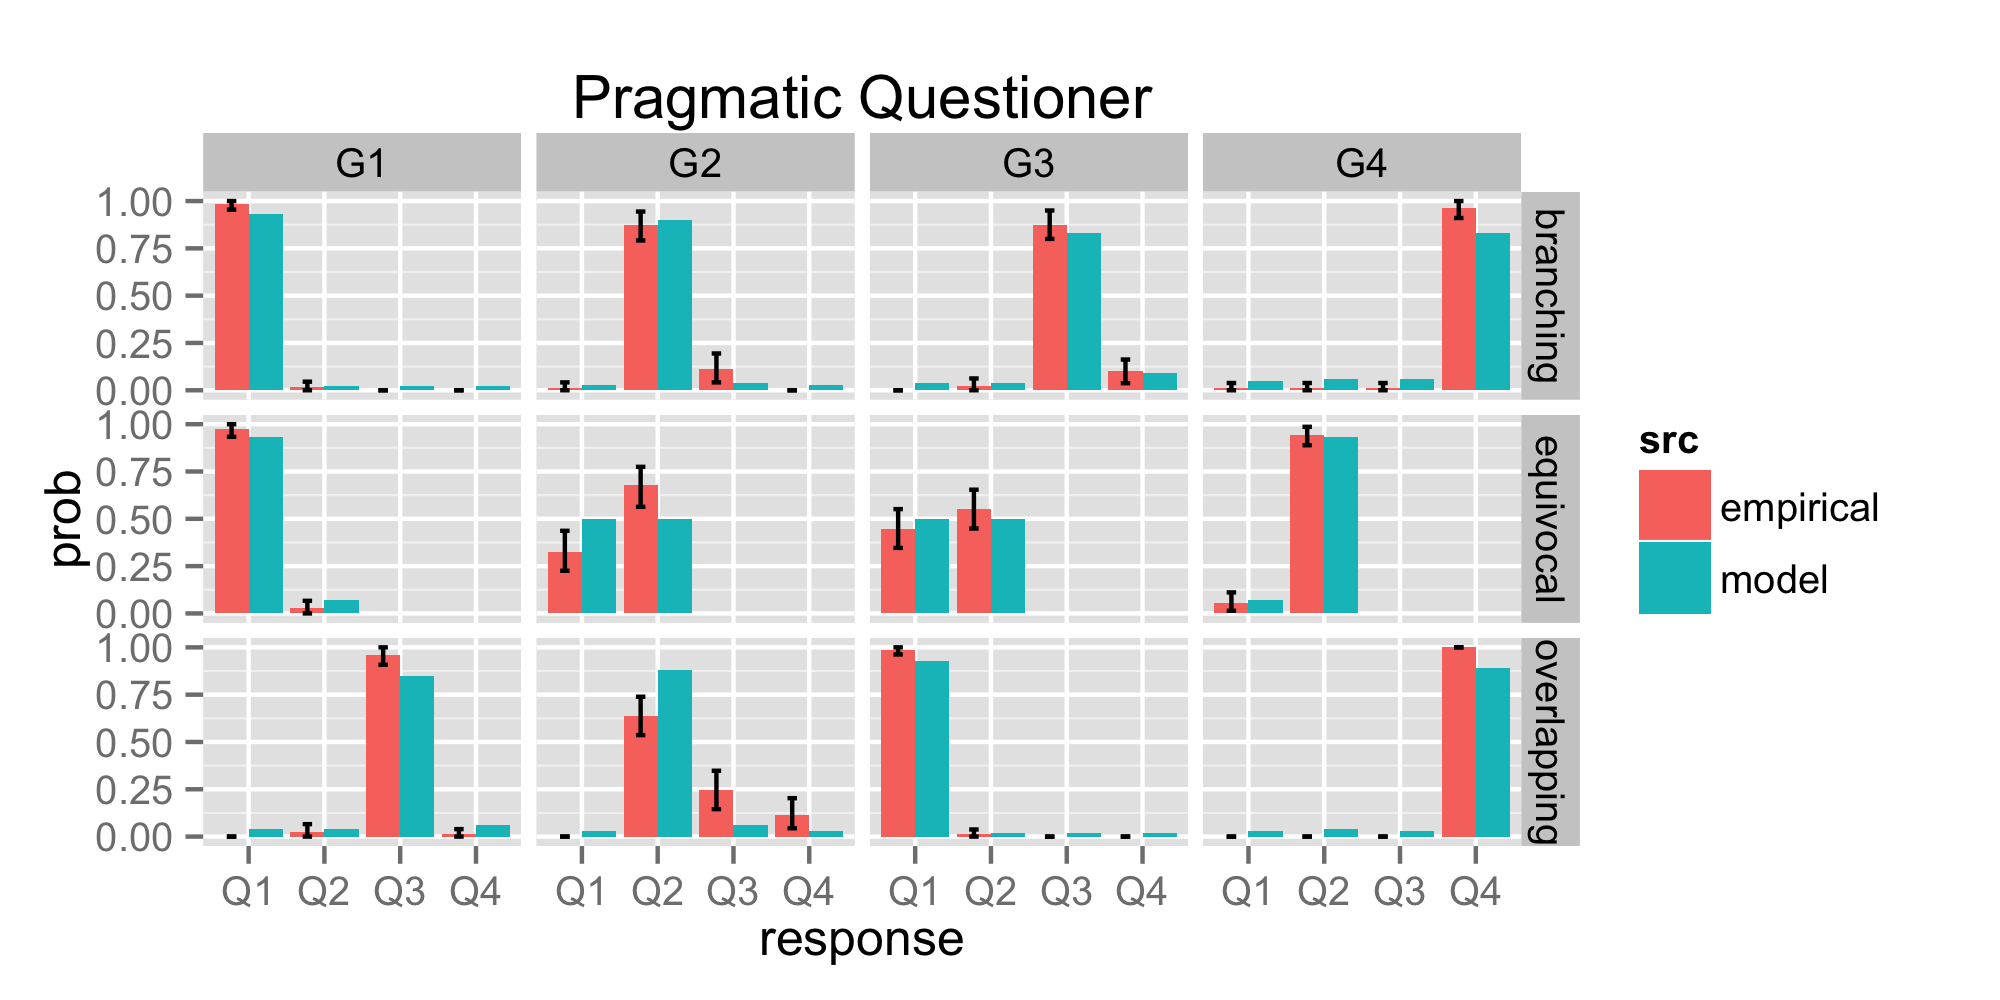
\includegraphics[scale = .25]{Exp4QuestResults}
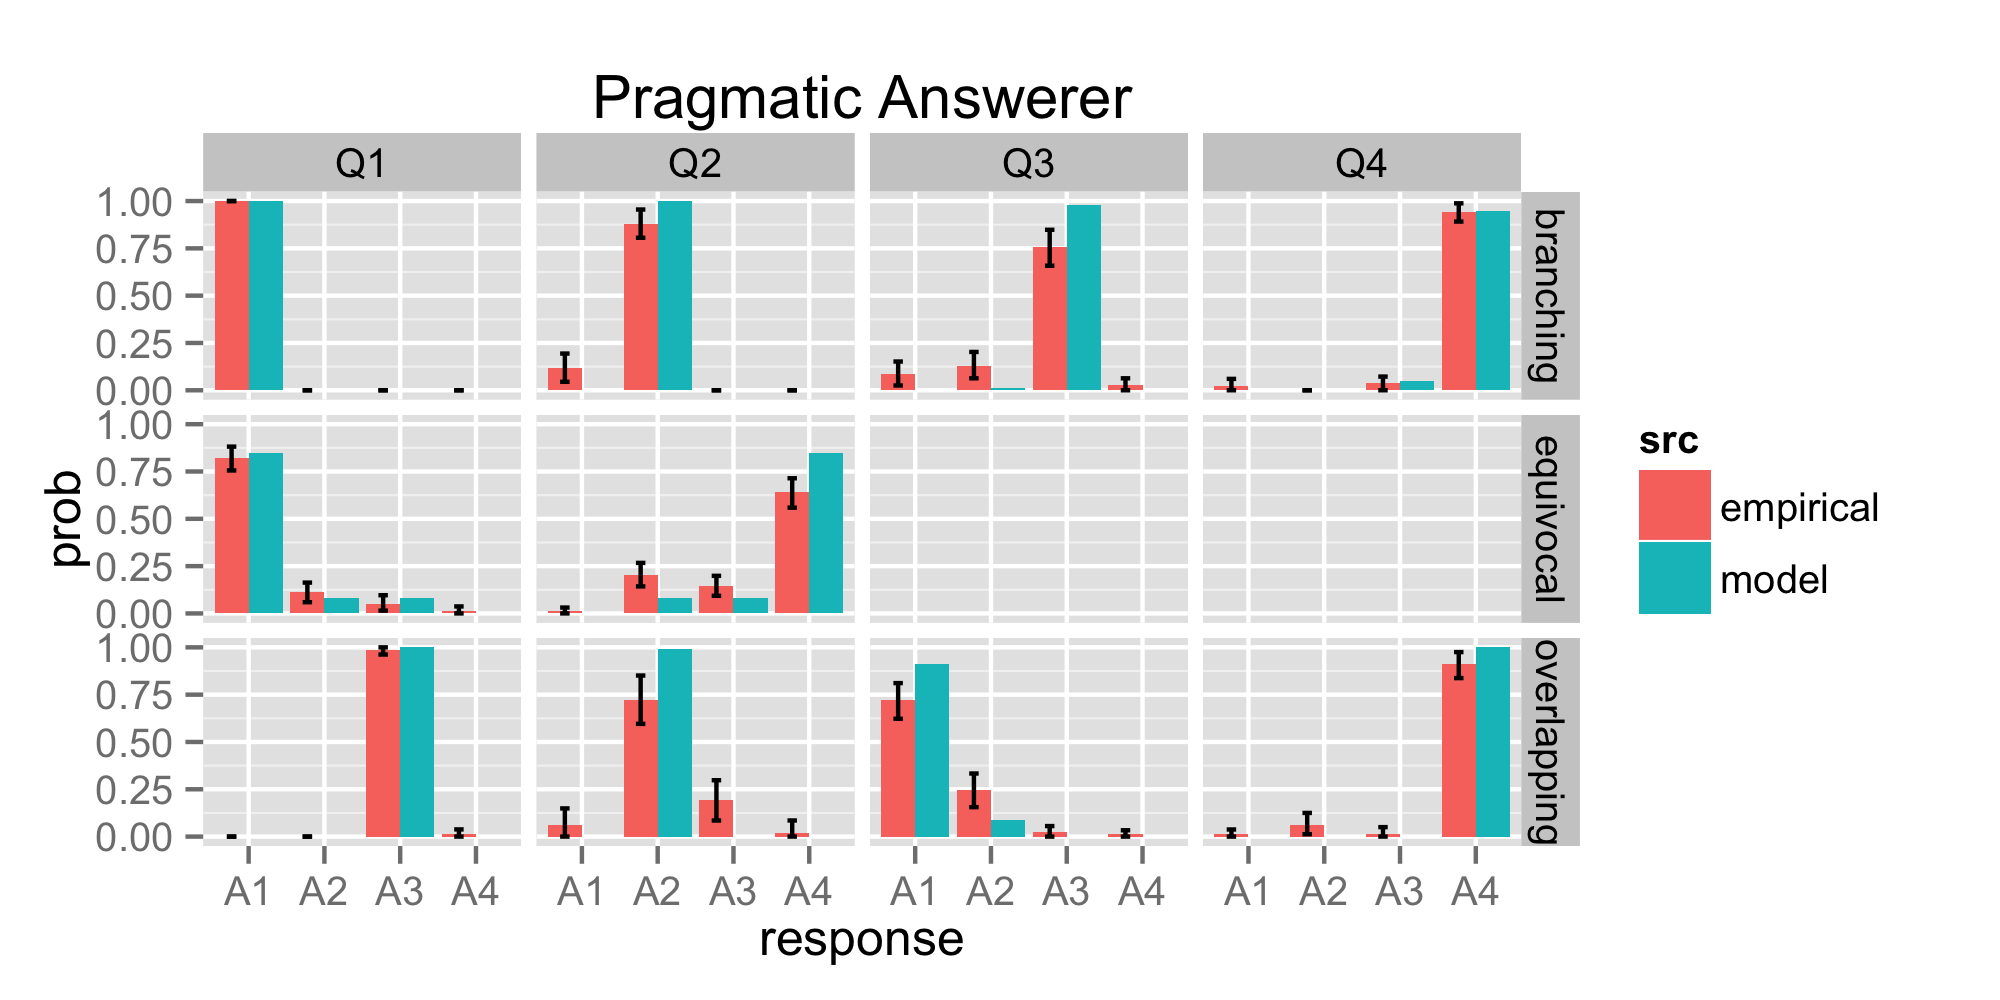
\includegraphics[scale = .25]{Exp4AnsResults}
\end{center}
\caption{Exp.~2 results and model fits, for the best-performing questioner (left) and answerer (right) models, collapsing over the different domains. Error bars represent bootstrapped 95\% confidence intervals.}
\label{fig:exp4res}
\end{figure*}

\subsubsection{Model comparison}

%
\begin{figure*}[t!]
\begin{center}
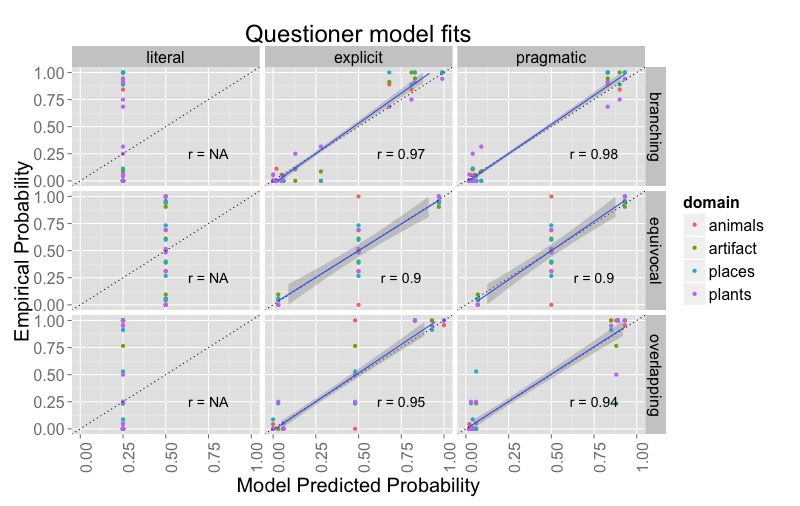
\includegraphics[scale=.57]{Exp4QuestFits.jpeg}
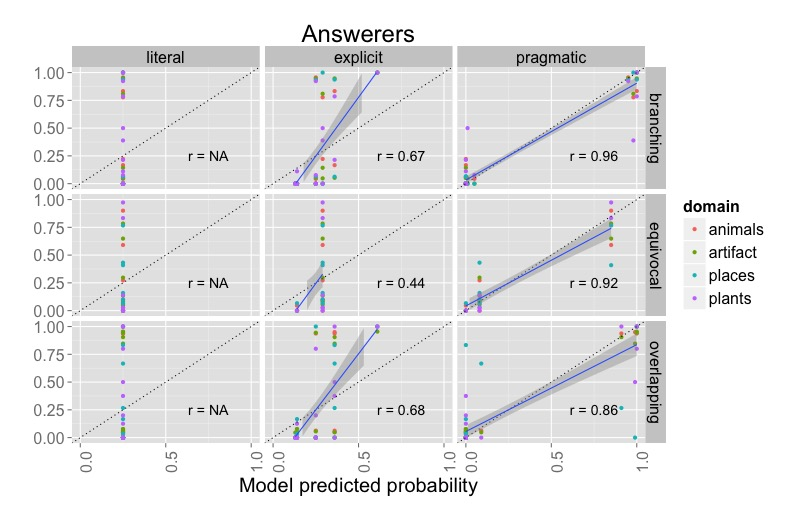
\includegraphics[scale=.57]{Exp4AnsFits.jpeg}
\end{center}
\caption{Full space of models, and their correlations with the data from Exp.~2, broken down by item and type.}
\label{fig:Exp4ModelSpace}
\end{figure*}
%

Model comparison was conducted in the same way as in Experiment 1. However, to avoid overfitting and to reduce the number of free parameters that would result from separately fitting rationality parameters for each item, we pool together data from all hierarchy structures and domains and fit the single rationality parameter for each model to jointly optimize model-data correlations across all items in this pooled dataset. 
%
\begin{figure*}[t!]
\begin{center}
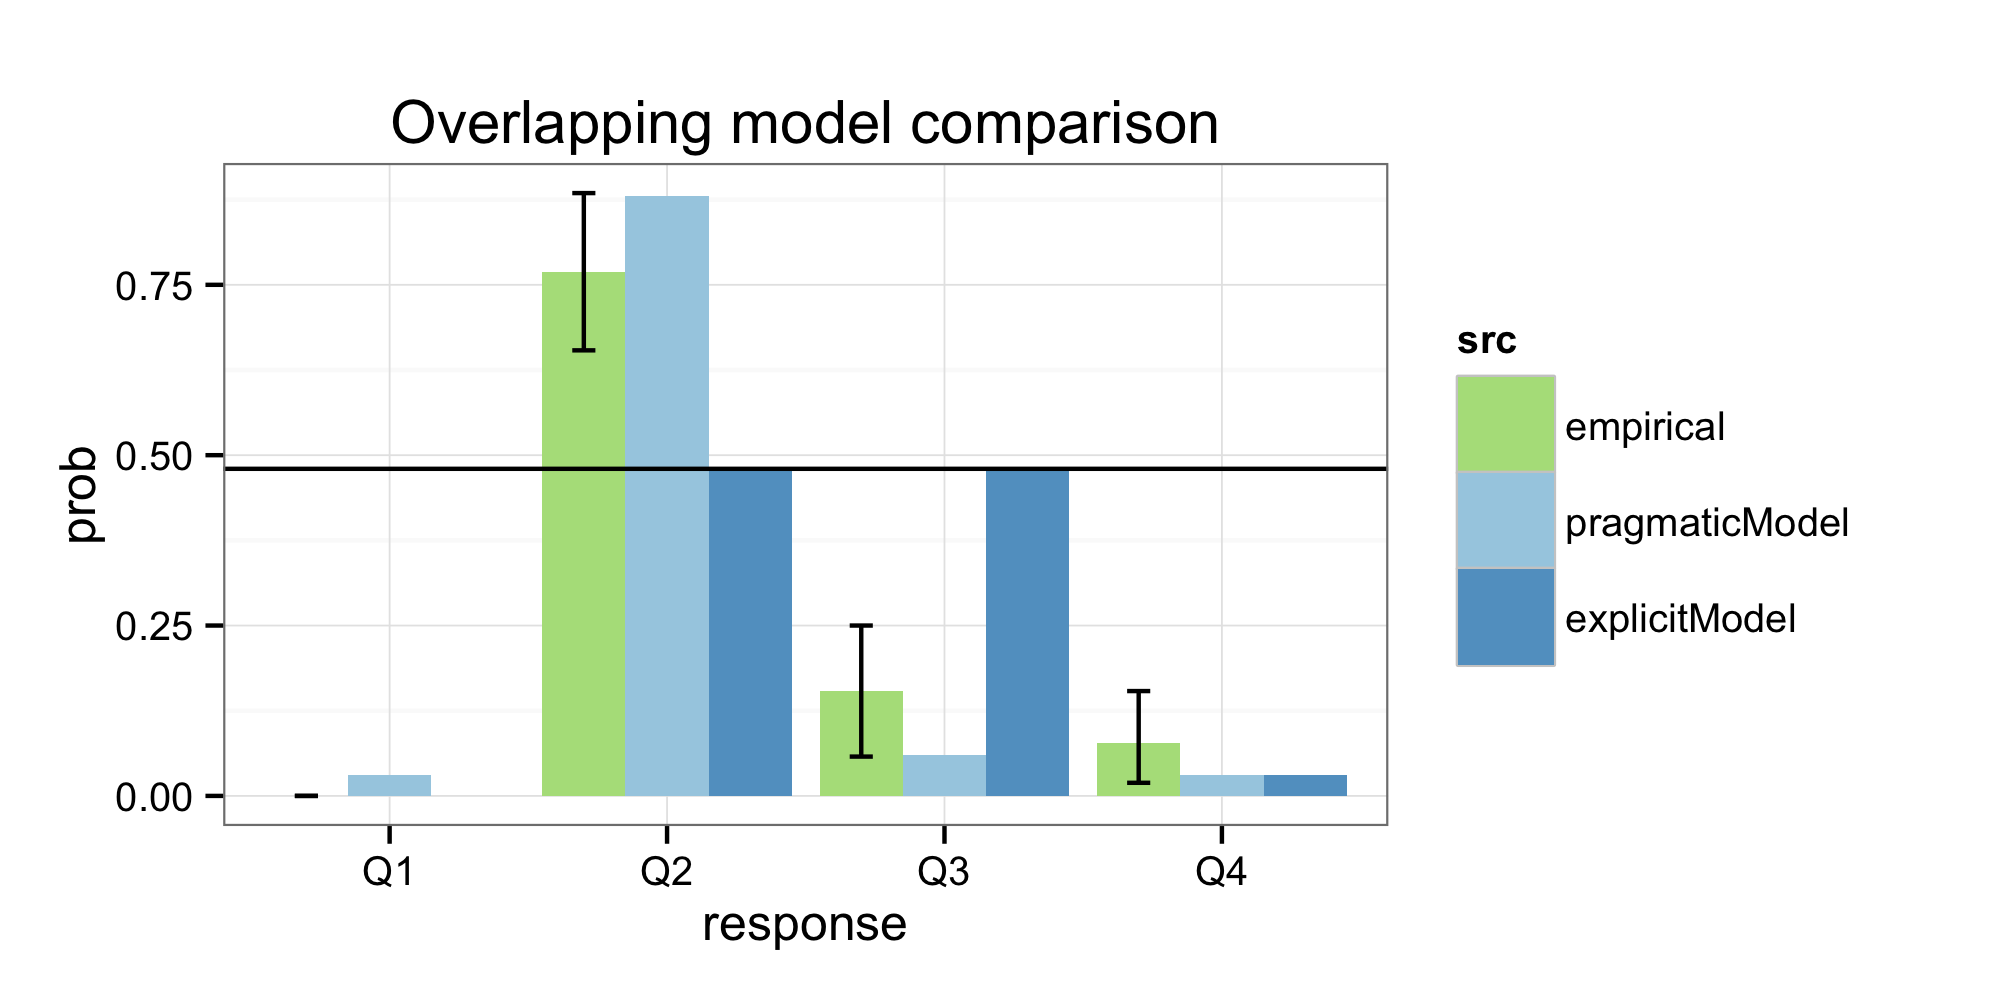
\includegraphics[scale=.25]{OverlappingModelComparison.png}
\end{center}
\vspace{-.5cm}
\caption{Full space of models, and their correlations with the data from Exp.~2, broken down by item and type.}
\label{fig:Exp4ZoomedIn}
\vspace{-.15cm}
\end{figure*}
%
These model-data fits, broken down by model level and hierarchy structure, are displayed in Figure \ref{fig:Exp4ModelSpace}. We can immediately rule out the literal answerer and literal questioner, which predict a uniform distribution of responses. We also find that the explicit answerer models fit the data significantly worse than the pragmatic answerer model in all hierarchy structures, with $r = 0.67$ compared to $r = 0.96$ in the `branching' hierarchy, $r = 0.44$ compared to $r = 0.92$ in the `equivocal' hierarchy, and $r = 0.68$ compared with $r = 0.86$ in the `overlapping' hierarchy, respectively. 

Turning to the questioner predictions, we again find that both explicit and pragmatic models provide excellent but essentially indistinguishable fits, with $r = 0.97$ compared with $0.98$ in the `branching' hierarchy, $r = 0.90$ compared with $r = 0.90$ in the `equivocal hierarchy', and $r = 0.95$ compared with $0.94$ in the `overlapping' hierarchy, respectively. 

However, because we designed the overlapping structure to provide a critical test for the questioner models, it is not the overall correlation we are interested in, it is the particular distribution of responses to ``G2'' (the ``house cat'' in the animal domain). Since ``house cat'' is not available as a question, the explicit model (as well as the heuristic strategy discussed above) predicts that the two parents, ``pet'' and ``cat'' will be equally likely. This happens because the explicit answerer would be equally likely to reveal the location of the house cat in response to ``pet'' and ``cat,'' which each have two children. 

The pragmatic questioner model, however, predicts that ``cat'' will be preferred over ``pet'', because the other child of ``cat'' -- the lion -- is pragmatically blocked by the pragmatic answerer. When the pragmatic answerer hears ``cat'' they reason that if the questioner's underlying goal were the ``lion'' they would have \emph{said} lion; because they didn't, they must mean the other cat. Thus, we have a pair of sharply distinguishable predictions: the explicit model predicts that ``pet'' and ``cat'' will be equally likely and the pragmatic model predicts an asymmetry where ``cat'' is the preferred label. 

In Figure \ref{fig:Exp4ZoomedIn}, we zoom in on this critical condition and display both models' predictions next to the empirical data, with bootstrapped 95\% confidence intervals. For these analyses, we excluded the `places' domain both because it was flagged as an outlier early in the analysis and because our stimulus design led to a confound in the `overlapping' condition, which we discuss further below. We find that the pragmatic model makes the correct qualitative prediction -- the mean probability of responding ``Q2'' ($p_{Q2} = 0.77, n = 52, 95\%\textrm{ bootstrapped CI }= [0.65, 0.88])$ in this condition is significantly different from the mean probability of responding ``Q3'' ($p_{Q3} = 0.15, n = 52, 05\% \textrm{ bootstrapped CI }=[0.06, 0.25]$), as predicted by the pragmatic model. We also see that it makes a relatively good quantitative prediction, with the predicted probability lying within the 95\% confidence interval of the empirical estimate for both the ``Q2'' and ``Q3'' responses. Recall that a single free parameter $\alpha$ for each model was fit to maximize correlations for the entire (pooled) dataset.




\subsubsection{Discussion}

We have replicated the results of Experiment 1, and shown that these results generalize to a wider range of domains and hierarchy structures. Additionally, we were able to distinguish between the pragmatic and explicit questioner models, finding that the pragmatic model is necessary to account for some critical aspects of the data. The ``place'' domain that we flagged as a potential outlier earlier in the results is the only domain that does not show the pattern of responses predicted by the pragmatic questioner model. This is likely due to the choice of images displayed to participants: the two ``parent'' nodes of the critical goal are ``bar'' and ``restaurant,'' and we represented the intersection of these two categories as a hotel lobby. However, the image we chose placed emphasis in the bar in the hotel, which may have biased participants toward the ``bar'' response instead of the ``restaurant response'' predicted by the pragmatic model. Including it does not change the statistical results, but we do not believe it is representative of questioner behavior. 

\todo[inline]{rdh: The next paragraph would naturally lead into another experiment where we elicit label priors and re-run our model with label fitness included -- I think I'd be happier with the paper if we had this...}
We also find that while overall fits are good, all our models fail to capture graded responses across different domains. This is especially striking in the `equivocal' condition where all our models predict a symmetry in questioner behavior for the two goals where the questions options are equally uninformative. Instead, we found a high degree of variability across domains. To some extent, this is expected from a model with only a single parameter fit for all domains simultaneously. We could have fit separate rationality parameters for each domain to capture domain-level differences. However, we expect that this variability can be accounted for in a more principled way by a prior over label fitness. In our data, `fish' was considered a better label for a picture of a pet goldfish than `pet' by 85\% of participants, even though both are technically true. When there is no pragmatic reason to favor one over the other, participants fall back on their label prior. If we ran a separate study to elicit this prior, we could simply plug the empirical priors into our model and naturally account for the variability across items without introducing additional free parameters. Alternatively, we could use Bayesian data analysis to infer these priors from question and answer response data. 

\section{General discussion}
\label{sec:gd}

We have presented evidence that answerer behavior is best described by a pragmatic model that \emph{does} reason about questioner intentions, using the question utterance as a signal. Our study provides a next step for previous QUD-based linguistic accounts by concretely specifying how an answerer may make such inferences via Bayesian conditioning. The superiority of pragmatic answerer predictions over the other answerer models was robust across all experiments. 

Questioner behavior, however, appeared to be more sensitive to the experimental set-up. In a single-player pilot version of Exp.~1, for example, we did not emphasize certain aspects of the game in the instructions, such as the fact that the answerer knows about the restricted answer set. Our data in this pilot experiment appeared to contain a mixture of explicit and pragmatic answerers and questioners (though other confounds were present in this version). We found the interactive, multi-player version of the task, used in this paper to be more robust to these minor variations. 

We also found that at least in certain scenarios like the overlapping hierarchy condition of Exp~.2, questioners systematically relied on higher-order pragmatic reasoning about what inferences an answerer would make about their own underlying goals when deciding what question to ask. Note that this behavior also could not be explained by the heuristic strategy raised in the earlier experiments: if questioners just ruled out labels that did not apply (e.g. ``lion''), they would have no mechanism for deciding between the two equally-good parent labels (``pet'' and ``cat'') to pick out their goal. It will ultimately be important to explore the mixture of explicit- and pragmatic-questioning across an even larger range of situations: these issues may be a product of our artificial game paradigm, or they may be reflective of real tendencies in language use, raising novel questions about audience design in question-answer behavior.

\todo[inline]{ndg: somewhere (discussion?) explore whether this notion of goals is enough to capture all kinds of questions.}

\todo[inline]{rdh: Address different ways of setting up model (e.g. fixed-point, Clark `joint project'?)}

\todo[inline]{rdh: discuss differences with van rooy more broadly?}

\todo[inline]{rdh: discuss issues with use of definite article in question: `the animal?' or `that animal?' presupposes the existence of a salient animal, while `an animal?' or `one of the animals?' would not.}

\todo[inline]{rdh: discuss different ways we can relax assumptions of the model to capture different kinds of effects. e.g. we implicitly assume knowledge is fixed and in common ground. What if there was uncertainty over what the other person knew? Could we then model teacher-student interactions?}

\todo[inline]{rdh: discuss how our assumptions may or may not really scale up, e.g. how do you possibly populate the space of QUDs outside of our game context or a rigid social interaction like asking for the time or buying something? Topic modeling? How do you populate the space of alternative questions or alternative answers? Conditional frequency in some corpus?}

\todo[inline]{ndg: random note about politeness: we often use more words than necessary, just to avoid seeming curt. for instance i'd bet a lot of the 'yes' answers in the credit cards experiment are actually something like 'yes, we do'. one way to think about this is that the answerers relative balance between cost and helpfulness (roughly how much they care) is unknown to the questioner, and questioners will infer this. thus the answerer will choose answers partly to signal that they value helping.\\rdh: putting this in general discussion as an example of another way we could lift aspects of the model to be inferred. }

Perhaps the most important formal advance of the models considered here is to move the Rational Speech Act framework beyond interpretation of single utterances (in context), to consider the dynamics of simple dialogs (albeit consisting of a single question and its answer). 
Doing so requires replacing the immediate motive to convey true information with the more distant motive to provoke useful information from one's interlocutor. On the answerer side, sophisticated inference was required to account for the implicit interests of the questioner. This provides a useful connection to current game-theoretic and decision-theoretic models \cite{VogelBodoiaPottsJurafsky13_GricePOMDP, VanRooy03_QuestioningDecisionProblems}, which also emphasize the importance of goals and speaker beliefs in communication but emphasize less the complex interplay of inference between questioner and answerer.


%One additional consideration is the apparent failure of any of our models to capture questioner behavior in the ``equivocal'' hierarchy. All models we considered predicted that there would be no preference between the ``fish'' and ``pet'' labels when attempting to find an object at the intersection of these labels (e.g. the ``goldfish''). In fact, nearly all participants chose the label ``fish!'' We expect that this is due to prior beliefs about \emph{label fitness}: for any object-label pair, we can measure how willing a typical language user would be to apply the label to the object. While technically the goldfish is both a fish and a pet, it is much more likely to be called a ``fish'' in a vacuum. In future work, we intend to extend our model to allow for \emph{mixtures} of QUDs, such that the interpretation of a question word takes label fitness into account.

While the artificiality of our question-answer game may distance the behavior of participants from the natural use of language, there are also some benefits to this design. In particular, it is easy in this setting to control the exact space of questions, goals, and answers. While the restrictions on question space may seem peculiar, it is directly motivated by conversational scenarios in everyday usage which feature restrictions on the set of things one can ask about, due to politeness, salience, time cost, and other factors. In future work, we will explore the extent to which the proposed model can scale up to extended dialogues, and other more naturalistic language settings. To deal with dialogues lasting longer than a single exchange, for instance, we must specify the way in which the contributions of questioner and answerer affect the \emph{context} in which later utterances operate. 

Humans are experts at inferring the intentions of other agents from their actions \cite{TomaselloCarpenter___Moll05_IntentionsCulturalCognition}. Given simple motion cues, for example, we are able to reliably discern high-level goals such as chasing, fighting, courting, or playing \cite{BarrettToddMillerBlythe05_IntentionFromMotionCues, HeiderSimmel44_Animacy}. Experiments in psycholinguistics have shown that this expertise extends to speech acts.  Behind every question lies a goal or intention. This could be an intention to obtain an explicit piece of information (``Where can I get a newspaper?''), signal some common ground (``Did you see the game last night?''), test the answerer's knowledge (``If I add these numbers together, what do I get?''), politely request the audience to take some action (``Could you pass the salt?''), or just to make open-ended small talk (``How was your weekend?''). These wildly different intentions seem to warrant different kinds of answers%, even if the explicit question is expressed using the same words
. By formalizing the computational process by which answerers infer these different intentions, our model framework provides a unifying way to accommodate this diversity.  % If questions themselves are informative, we must ask them carefully.


\bibliography{qa}
\bibliographystyle{apacite}


\end{document}  
